TODO REFINE
- don't use resize population and always use normal size to be consistent and feed random population as random parameter
- use TimeRange and UnitRange consistently everywhere
- WORDING: don't use replications in terms of QuickCheck! we test properties with random test-cases
- IMPROVE EXPLANATION: more explanations, its too flat, code straight in the face, prepare it gently as it is not directly clear what the intention is. discuss it more generally, otherwise it reads like an advanced technical report and not like a thesis.
- explain more how and why and when we use cover and checkCoverage. Also when using cover we cannot use random model parameters as it changes distributions
- only use cover with/without checkCoverage instead of maxFailPercent => rework sugarscape hypotheses chapter; need not much change only remove maxFailPercent and use cover and run all cases again.

\bigskip

\section{Introduction}
There exists a large number of simulation packages which allow the convenient creation of System Dynamics simulations by straight-forward visual diagram creation. One simply creates stocks and flows, connects them, specifies the flow-rates and initial parameters and then runs the model. An example for such a visual diagram creation in the simulation package AnyLogic can be seen in Figure \ref{fig:sir_stockflow_diagram}.

\begin{figure}
	\centering
	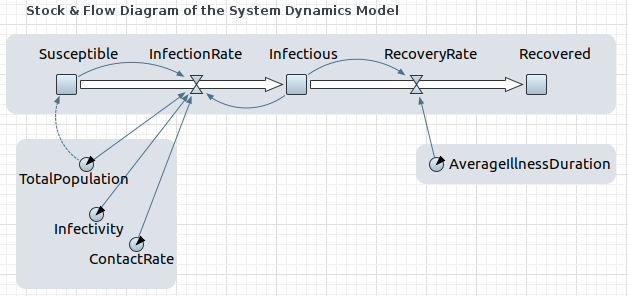
\includegraphics[width=.5\textwidth, angle=0]{./fig/SIR_SD_STOCKFLOW_DIAGRAMM.png}
	\caption{Visual System Dynamics Diagram of the SIR model in AnyLogic Personal Learning Edition 8.3.1.}
	\label{fig:sir_stockflow_diagram}
\end{figure}

Still, implementing System Dynamics directly in code is not as straight forward and involves numerical integration which can be quite tricky to get right. Thus, the aim of this paper is to look into how System Dynamics models can be implemented in code correctly without the use of a simulation package. We use the well known SIR model \cite{kermack_contribution_1927} from epidemiology to demonstrate our approach.

Our language of choice is Haskell because it emphasises a declarative programming style in which one describes \textit{what} instead of \textit{how} to compute. Further it allows to rule out interference with non-deterministic influences or side-effects already at compile-time. This is of fundamental importance for System Dynamics because it behaves completely deterministic and involves no stochastics or non-determinism whatsoever. Also, we make use of Functional Reactive Programming which allows to express continuous-time systems in a functional way. 

We show that by this approach we can arrive at correct-by-construction implementations of System Dynamic models. This means that the correctness of the code is obvious because we have closed the gap between the model specification and its implementation. Thus, the contribution of the paper is the demonstration of how to implement correct-by-construction System Dynamics simulations using Haskell and Functional Reactive Programming.

\section*{Property-Based Testing}
\label{sec:proptesting}

Property-based testing allows to formulate \textit{functional specifications} in code which then a property-based testing library tries to falsify by \textit{automatically} generating test-data, covering as much cases as possible. When a case is found for which the property fails, the library then reduces the test-data to its simplest form for which the test still fails e.g. shrinking a list to a smaller size. It is clear to see that this kind of testing is especially suited to ABS, because we can formulate specifications, meaning we describe \textit{what} to test instead of \textit{how} to test. Also the deductive nature of falsification in property-based testing suits very well the constructive and exploratory nature of ABS. Further, the automatic test-generation can make testing of large scenarios in ABS feasible because it does not require the programmer to specify all test-cases by hand, as is required in e.g. traditional unit tests.

Property-based testing was introduced in \cite{claessen_quickcheck_2000,claessen_testing_2002} where the authors present the QuickCheck library in Haskell, which tries to falsify the specifications by \textit{randomly} sampling the test space. We argue, that the stochastic sampling nature of this approach is particularly well suited to ABS, because it is itself almost always driven by stochastic events and randomness in the agents behaviour, thus this correlation should make it straightforward to map ABS to property-testing.
%The main challenge when using QuickCheck, as will be shown later, is to write \textit{custom} test-data generators for agents and the environment which cover the space sufficiently enough to not miss out on important test-cases.
According to the authors of QuickCheck \textit{"The major limitation is that there is no measurement of test coverage."} \cite{claessen_quickcheck_2000}. Although QuickCheck provides help to report the distribution of test-cases it is not able to measure the coverage of tests in general. This could lead to the case that test-cases which would fail are never tested because of the stochastic nature of QuickCheck. Fortunately, the library provides mechanisms for the developer to measure coverage in specific test-cases where the data and its (expected) distribution is known to the developer. This is a powerful tool for testing randomness in ABS as will be shown in subsequent chapters.

\medskip

As a remedy for the potential coverage problems of QuickCheck, there exists also a deterministic property-testing library called SmallCheck \cite{runciman_smallcheck_2008}, which instead of randomly sampling the test-space, enumerates test-cases exhaustively up to some depth. It is based on two observations, derived from model-checking, that (1) \textit{"If a program fails to meet its specification in some cases, it almost always fails in some simple case"} and (2) \textit{"If a program does not fail in any simple case, it hardly ever fails in any case} \cite{runciman_smallcheck_2008}. This non-stochastic approach to property-based testing might be a complementary addition in some cases where the tests are of non-stochastic nature with a search-space  too large to test manually by unit tests but small enough to enumerate exhaustively. The main difficulty and weakness of using SmallCheck is to reduce the dimensionality of the test-case depth search to prevent combinatorial explosion, which would lead to exponential number of cases. Thus one can see QuickCheck and SmallCheck as complementary instead of in opposition to each other.

\subsection*{A brief overview of QuickCheck}
To give a rough idea on how property-based testing works in Haskell, we give a few examples of property-tests on lists, which are directly expressed as functions in Haskell. Such a function has to return a \textit{Bool} which indicates \textit{True} in case the test succeeds or \textit{False} if not and can take input arguments which data is automatically generated by QuickCheck.

\begin{HaskellCode}
-- concatenation operator (++) is associative
append_associative :: [Int] -> [Int] -> [Int] -> Bool
append_associative xs ys zs = (xs ++ ys) ++ zs == xs ++ (ys ++ zs)

-- the reverse of a reversed list is the original list
reverse_reverse :: [Int] -> Bool
reverse_reverse xs = reverse (reverse xs) == xs

-- reverse is distributive over concatenation (++)
-- this test fails for explanatory reasons, for a correct 
-- property xs and ys need to be swapped on the right-hand side!
reverse_distributive :: [Int] -> [Int] -> Bool
reverse_distributive xs ys = reverse (xs ++ ys) == reverse xs ++ reverse ys

-- running the tests
main :: IO ()
main = do
  quickCheck append_associative
  quickCheck reverse_reverse
  quickCheck reverse_distributive
\end{HaskellCode}

When we run the tests using \textit{main}, we get the following output:

\begin{verbatim}
+++ OK, passed 100 tests.
+++ OK, passed 100 tests.
*** Failed! Falsifiable (after 5 tests and 6 shrinks):    
[0]
[1]
\end{verbatim}

We see that QuickCheck generates 100 test-cases for each property-test and it does this by generating random data for the input arguments. Note that we have not specified any data for our input arguments; QuickCheck is able to provide a suitable data-generator through type-inference: for lists and all the existing Haskell types like Int there exist custom generators already.

QuickCheck generates 100 test-cases by default and requires all to pass - if there is a test-case which fails, the overall property-test fails and QuickCheck shrinks the input to a minimal size for which the case still fails and reports it as a counter example. This is the case in the last property-test \textit{reverse\_distributive} which is wrong as \textit{xs} and \textit{ys} need to be swapped on the right-hand side. In this run, QuickCheck found a counter-example to the property after 5 tests and applied 6 shrinks to find the minimal failing example of \textit{xs = [0]} and \textit{ys = [1]}. If we swap \textit{xs} and \textit{ys}, the property-test passes 100 test-cases just like the other two did. Note that it is possible to configure QuickCheck to generate more or less random test-cases, which can be used to increase the coverage if the sampling space is quite large - this will become useful later.

\subsubsection*{Properties and Generators}
TODO: property
TODO: label
TODO: ==>
TODO: generators

\subsubsection*{Coverage}
TODO: cover with checkCoverage


\section*{Testing ABS implementations}
\label{sec:testingABS}
TODO: this is a rather weak section, polish it by writing more general about it and how we can use property-based testing for it. if i cannot come up with something more substantial simply scrap it

Generally we need to distinguish between two types of testing / verification in ABS.

\begin{enumerate}
	\item Testing / verification of models for which we have real-world data or an analytical solution which can act as a ground-truth - examples for such models are the SIR model, stock-market simulations, social simulations of all kind.
	\item Testing / verification of models which are of exploratory nature, inspired by real-world phenomena but for which no ground-truth per se exists - examples for such models is the Sugarscape \cite{epstein_growing_1996} or Agent\_Zero model \cite{epstein_agent_zero:_2014}.
\end{enumerate}

The baseline is that either one has an analytical model as the foundation of an agent-based model or one does not. In the former case, e.g. the SIR model, one can very easily validate the dynamics generated by the simulation to the one generated by the analytical solution through System Dynamics. In the latter case one has basically no idea or description of the emergent behaviour of the system prior to its execution e.g. SugarScape. In this case it is important to have some hypothesis about the emergent property / dynamics. The question is how verification / validation works in this setting as there is no formal description of the expected behaviour: we don't have a ground-truth against which we can compare our simulation dynamics.

One distinguishes between black-box and white-box verification where in white-box verification one looks directly at code and reasons about it whereas in black-box verification one generally feeds input to the software / functions / methods and compares it to expected output. Black-box verification is our primary concern in this chapter as property-based testing is an instance of black-box verification. In the case of ABS we have the following levels of black-box tests \cite{nguyen_testing_2011}: %%Although the work on TDD is scarce in ABS, there exists quite some research on applying TDD and unit testing to multi-agent systems (MAS). Although MAS is a different discipline than ABS, the latter one has derived many technical concepts from the former one, thus testing concepts applied to MAS might also be applicable to ABS. The paper \cite{nguyen_testing_2011} is a survey of testing in MAS. It distinguishes between unit-tests of parts that make up an agent, agent tests which test the combined functionality of parts that make up an agent, integration tests which test the interaction of agents within an environment and observe emergent behaviour, system tests which test the MAS as a system running at the target environment and acceptance test in which stakeholders verify that the software meets their goal. Although not all ABS simulations need acceptance and system tests, still this classification gives a good direction and can be directly transferred to ABS. 
\begin{enumerate}
	\item Isolated and interacting agent behaviour parts - test the individual parts which make up the agent behaviour under given inputs. Also test if interaction between agents are correct. For this we can use traditional unit-tests as shown by \cite{collier_test-driven_2013} and also property-based testing as we will show in the case studies.
	\item Simulation dynamics - compare emergent dynamics of the ABS as a whole under given inputs to an analytical solution or real-world dynamics in case there exists some, using statistical tests. We see this type of tests conceptually as property-tests as well because we are testing properties of the model / simulation as we will see in the case-studies. Technically speaking we can use both unit and property-based tests to implement them - conceptually they are property-tests.
	\item Hypotheses - test whether hypotheses about the model are valid or invalid. This is very similar to the previous point but without comparing it to analytical solutions or real-world dynamics but only to some hypothetical values.
\end{enumerate}

TODO: make it clear that we focus on the event-driven SIR implemention only. why? because of its more interesting nature and because its concepts are also applicable to the sugarscape as well. the time-driven implementation will be shortly discussed in releveant sections.

\chapter{Testing Agent specifications}
\label{ch:agentspec}

In this chapter we are showing how to use QuickCheck to encode full agent-specifications directly in code as property-tests. These properties serve then both as formal specification and tests at the same time - a fundamental strength of property-based testing, not possible with unit-testing in this strong expressive form. Besides the high expressivity, QuickCheck also allows us to state statistical coverage for certain cases, which allows to express statistical properties of the agents behaviour, something also not directly possible with unit-testing. This is a very strong indication that property-based testing is a natural fit to test agent-based simulation. We discuss both time- and event-driven  implementations of the agent-based SIR model as introduced in Chapter \ref{sec:sir_model}.

\section{Event-driven specification}
In this section we present how QuickCheck can be used to test event-driven agents by expressing their \textit{specification} as property tests in the case of the event-driven SIR implementation from chapter \ref{sec:eventdriven_basics}.

In general, testing event-driven agents is fundamentally different and more complex than testing time-driven agents, as their interface surface is generally much larger. Events form the input to the agents to which they react with new events where the dependencies between those can be quite complex and deep. Using property-based testing we can encode the invariants and end up with an actual specification of their behaviour, acting as documentation, regression test within a TDD and property tests.

Note that the concepts presented here are applicable with slight adjustments to the Sugarscape implementation as well but we focused on the SIR one as its specification is shorter and does not require as much in-depth details. % - after all we are interested in deriving concepts, not dealing with specific technicalities.

With event-driven ABS, a good starting point in specifying and testing the system, is simply relating the input events to expected output events. In the SIR implementation we have only three events, making it feasible to give a full formal specification. The Sugarscape implementation has more than 16 events, which makes it much harder to test it with sufficient coverage, giving a good reason to primarily focus on the SIR implementation for explanatory purposes.

\subsection{Deriving the specification}
We start by giving the full \textit{specification} of the susceptible, infected and recovered agent by stating the input-to-output event relations. The susceptible agent is specified as follows:

\begin{enumerate}
	\item \texttt{MakeContact} - if the agent receives this event it will output $\beta$ \texttt{Contact ai Susceptible} events, where \texttt{ai} is the agents own id. The events have to be scheduled immediately without delay, thus having the current time as scheduling timestamp. The receivers of the events are uniformly randomly chosen from the agent population. The agent doesn't change its state, stays \texttt{Susceptible} and does not schedule any other events than the ones mentioned.
	
	\item \texttt{Contact \_ Infected} - if the agent receives this event there is a chance of uniform probability $\gamma$ (infectivity) that the agent becomes \texttt{Infected}. If this happens, the agent will schedule a \texttt{Recover} event to itself into the future, where the time is drawn randomly from the exponential distribution with $\lambda = \delta$ (illness duration). If the agent does not become infected, it will not change its state, stays \texttt{Susceptible} and does not schedule any events.
	
	\item \texttt{Contact \_ \_} or \texttt{Recover} - if the agent receives any of these other events it will not change its state, stays \texttt{Susceptible} and does not schedule any events.
\end{enumerate}

This specification implicitly covers that a susceptible agent can never transition from a \texttt{Susceptible} to a \texttt{Recovered} state within a single event as it can only make the transition to \texttt{Infected} or stay \texttt{Susceptible}. The infected agent is specified as follows:

\begin{enumerate}
	\item \texttt{Recover} - if the agent receives this, it will not schedule any events and make the transition to the \texttt{Recovered} state.
	
	\item \texttt{Contact sender Susceptible} - if the agent receives this, it will reply immediately with \texttt{Contact ai Infected} to \textit{sender}, where \texttt{ai} is the infected agents' id and the scheduling timestamp is the current time. It will not schedule any events and stays \texttt{Infected}.
	
	\item In case of any other event, the agent will not schedule any events and stays \texttt{Infected}.
\end{enumerate}

This specification implicitly covers that an infected agent never goes back to the \texttt{Susceptible} state as it can only make the transition to \texttt{Recovered} or stay \texttt{Infected}. From the specification of the susceptible agent it becomes clear that a susceptible agent who became infected, will always recover as the transition to \texttt{Infected} includes the scheduling of \texttt{Recovered} to itself. 

\medskip

The \textit{recovered} agent specification is very simple. It stays \texttt{Recovered} forever and does not schedule any events.

\medskip

The question is now how to put these into a property test with QuickCheck. We focus on the susceptible agent, as it it the most complex one, which concepts can then be easily applied to the other two. Generally speaking, we create a random \textit{susceptible} agent and a random event, feed it to the agent to get the output and check the invariants accordingly to input and output. % In the specification there are stated three probabilities regarding $\beta$ (contact rate), $\gamma$ (infectivity) and $\delta$ (illness duration). We will only check one, $\gamma$ (infectivity) using the coverage features of QuickCheck and write additional property tests for the other two. The reason for that is, that checking $\gamma$ is natural with the invariant checking whereas the others need a slightly different approach and are more obviously stated in separate property tests.

\subsection{Encoding invariants}
We start by encoding the invariants of the susceptible agent directly into Haskell, implementing a function which takes all necessary parameters and returns a \texttt{Bool} indicating whether the invariants hold or not. The encoding is straightforward when using pattern matching and it nearly reads like a formal specification due to the declarative nature of functional programming.

\begin{HaskellCode}
susceptibleProps :: SIREvent              -- ^ Random event sent to agent
                 -> SIRState              -- ^ Output state of the agent
                 -> [QueueItem SIREvent]  -- ^ Events the agent scheduled
                 -> AgentId               -- ^ Agent id of the agent
                 -> Bool
-- received Recover => stay Susceptible, no event scheduled
susceptibleProps Recover Susceptible es _ = null es
-- received MakeContact => stay Susceptible, check events
susceptibleProps MakeContact Susceptible es ai
  = checkMakeContactInvariants ai es cor 
-- received Contact _ Recovered => stay Susceptible, no event scheduled
susceptibleProps (Contact _ Recovered) Susceptible es _ = null es
-- received Contact _ Susceptible => stay Susceptible, no event scheduled
susceptibleProps (Contact _ Susceptible) Susceptible es _  = null es
-- received Contact _ Infected, didn't get Infected, no event scheduled
susceptibleProps (Contact _ Infected) Susceptible es _ = null es
-- received Contact _ Infected AND got infected, check events
susceptibleProps (Contact _ Infected) Infected es ai
  = checkInfectedInvariants ai es
-- all other cases are invalid and result in a failed test case
susceptibleProps _ _ _ _ = False
\end{HaskellCode}

Next, we give the implementation for the \texttt{checkMakeContactInvariants} and \texttt{checkInfectedInvariants} functions. The function \texttt{checkMakeContactInvariants} encodes the invariants which have to hold when the susceptible agent receives a \texttt{MakeContact} event. The \texttt{checkInfectedInvariants} function encodes the invariants which have to hold when the susceptible agent got \texttt{Infected}. Both implementations read like a formal specification, again thanks to the declarative nature of functional programming and pattern matching:

\begin{HaskellCode}
checkInfectedInvariants :: AgentId              -- ^ Agent id of the agent 
                        -> [QueueItem SIREvent] -- ^ Events the agent scheduled
                        -> Bool
checkInfectedInvariants sender 
  -- expect exactly one Recovery event
  [QueueItem receiver (Event Recover) t'] 
  -- receiver is sender (self) and scheduled into the future
  = sender == receiver && t' >= t 
-- all other cases are invalid
checkInfectedInvariants _ _ = False
\end{HaskellCode}

The \texttt{checkMakeContactInvariants} is a bit more complex but reads as a formal specification as well:

\begin{HaskellCode}
checkMakeContactInvariants :: AgentId              -- ^ Agent id of the agent 
                           -> [QueueItem SIREvent] -- ^ Events the agent scheduled
                           -> Int                  -- ^ Contact Rate
                           -> Bool
checkMakeContactInvariants sender es contactRate
    -- make sure there has to be exactly one MakeContact event and
    -- exactly contactRate Contact events
    = invOK && hasMakeCont && numCont == contactRate
  where
    (invOK, hasMakeCont, numCont) 
      = foldr checkMakeContactInvariantsAux (True, False, 0) es

    checkMakeContactInvariantsAux :: QueueItem SIREvent 
                                  -> (Bool, Bool, Int)
                                  -> (Bool, Bool, Int)
    checkMakeContactInvariantsAux 
        (QueueItem (Contact sender' Susceptible) receiver t') (b, mkb, n)
      = (b && sender == sender'   -- sender in Contact must be self
           && receiver `elem` ais -- receiver of Contact must be in agent ids
           && t == t', mkb, n+1)  -- Contact event is scheduled immediately
    checkMakeContactInvariantsAux 
        (QueueItem MakeContact receiver t') (b, mkb, n) 
      = (b && receiver == sender  -- receiver of MakeContact is agent itself
           && t' == t + 1         -- MakeContact scheduled 1 timeunit into future
           &&  not mkb, True, n)  -- there can only be one MakeContact event
    checkMakeContactInvariantsAux _ (_, _, _) 
      = (False, False, 0)         -- other patterns are invalid
\end{HaskellCode}

What is left is to actually write a property test using QuickCheck. We are making heavy use of random parameters to express that the properties have to hold invariant of the model parameters. We make use of additional data generator modifiers: \texttt{Positive} ensures that the value generated is positive; \texttt{NonEmptyList} ensures that the randomly generated list is not empty.

\begin{HaskellCode}
prop_susceptible_invariants :: Positive Int         -- ^ Contact rate (beta)
                            -> Probability          -- ^ Infectivity (gamma)
                            -> Positive Double      -- ^ Illness duration (delta)
                            -> Positive Double      -- ^ Current simulation time
                            -> NonEmptyList AgentId -- ^ population agent ids
                            -> Gen Property
prop_susceptible_invariants 
  (Positive beta) (P gamma) (Positive delta) (Positive t) (NonEmpty ais) = do
  -- generate random event, requires the population agent ids
  evt <- genEvent ais
  -- run susceptible random agent with given parameters
  (ai, ao, es) <- genRunSusceptibleAgent beta gamma delta t ais evt
  -- check properties
  return $ property $ susceptibleProps evt ao es ai
\end{HaskellCode}

When running this property test all 100 test cases pass. Due to the large random sampling space with 5 parameters, we increase the number of test cases to generate to 100,000 - still all test cases pass.

\subsection{Encoding transition probabilities}
In the specifications above there are probabilistic state transitions, for example an infected agent \textit{will} recover after a given time, which is randomly distributed with the exponential distribution. The susceptible agent \textit{might} become infected, depending on the events it receives and the infectivity ($\gamma$) parameter. We look now into how we can encode these probabilistic properties using the powerful \texttt{cover} and \texttt{checkCoverage} feature of QuickCheck.

\subsubsection{Susceptible agent}
We follow the same approach as in encoding the invariants of the susceptible agent but instead of checking the invariants, we compute the probability for each case. In this property test we cannot randomise the model parameters because this would lead to random coverage. This might seem like a disadvantage but we do not really have a choice here, still the model parameters can be adjusted arbitrarily and the property must hold. %Note that we do not provide the details of computing the probabilities of each input-to-output case as it is quite technical and of not much importance - it is only a matter of multiplication and divisions amongst the event-frequencies and model parameters.
We make use of the \texttt{cover} function together with \texttt{checkCoverage}, which ensures that we get a statistical robust estimate whether the expected percentages can be reached or not. Implementing this property test is then simply a matter of computing the probabilities and of case analysis over the random input event and the agents output.

\begin{HaskellCode}
...
case evt of 
  Recover -> 
    cover recoverPerc True 
     ("Susceptible receives Recover, expected " ++ show recoverPerc) True
...
\end{HaskellCode}

Note the usage pattern of \texttt{cover} where we unconditionally include the test case into the coverage class so all test cases pass. The reason for this is that we are just interested in testing the coverage, which is in fact the property we want to test. We could have combined this test into the previous one but then we couldn't have used randomised model parameters. For this reason, and to keep the concerns separated we opted for two different tests, which makes them also much more readable.

%\begin{HaskellCode}
%prop_susceptible_proabilities :: Positive Double      -- ^ Current simulation time
%                              -> NonEmptyList AgentId -- ^ Agent ids of the population
%                              -> Property
%prop_susceptible_proabilities (Positive t) (NonEmpty ais) = checkCoverage (do
%  -- fixed model parameters, otherwise random coverage
%  let cor = 5
%      inf = 0.05
%      ild = 15.0
%
%   -- compute distributions for all cases
%  let recoverPerc       = ...
%      makeContPerc      = ...
%      contactRecPerc    = ...
%      contactSusPerc    = ...
%      contactInfSusPerc = ...
%      contactInfInfPerc = ...
%
%  -- generate a random event
%  evt <- genEvent ais
%  -- run susceptible random agent with given parameters
%  (_, ao, _) <- genRunSusceptibleAgent cor inf ild t ais evt
%
%  -- encode expected distributions
%  return $ property $
%    case evt of 
%      Recover -> 
%        cover recoverPerc True 
%          ("Susceptible receives Recover, expected " ++ 
%           show recoverPerc) True
%      MakeContact -> 
%        cover makeContPerc True 
%          ("Susceptible receives MakeContact, expected " ++ 
%           show makeContPerc) True
%      (Contact _ Recovered) -> 
%        cover contactRecPerc True 
%          ("Susceptible receives Contact * Recovered, expected " ++ 
%           show contactRecPerc) True
%      (Contact _ Susceptible) -> 
%        cover contactSusPerc True 
%          ("Susceptible receives Contact * Susceptible, expected " ++ 
%           show contactSusPerc) True
%      (Contact _ Infected) -> 
%        case ao of
%          Susceptible ->
%            cover contactInfSusPerc True 
%              ("Susceptible receives Contact * Infected, stays Susceptible " ++
%               ", expected " ++ show contactInfSusPerc) True
%          Infected ->
%            cover contactInfInfPerc True 
%              ("Susceptible receives Contact * Infected, becomes Infected, " ++
%               ", expected " ++ show contactInfInfPerc) True
%          _ ->
%            cover 0 True "Impossible Case, expected 0" True
%\end{HaskellCode}

When running the property test we get the following output:

\begin{footnotesize}
\begin{verbatim}
+++ OK, passed 819200 tests:
33.3582% Susceptible receives MakeContact, expected 33.33%
33.2578% Susceptible receives Recover, expected 33.33%
11.1643% Susceptible receives Contact * Recovered, expected 11.11%
11.1096% Susceptible receives Contact * Susceptible, expected 11.11%
10.5616% Susceptible receives Contact * Infected, stays Susceptible, expected 10.56%
 0.5485% Susceptible receives Contact * Infected, becomes Infected, expected 0.56%
\end{verbatim}
\end{footnotesize}

After 819,200 (!) test cases QuickCheck comes to the conclusion that the distributions generated by the test cases reflect the expected distributions and passes the property test. We see that the values do not match exactly in some cases but by using sequential statistical hypothesis testing, QuickCheck is able to conclude that the coverage are statistically equal.

\subsubsection{Infected agent}
We want to write a property test which checks whether the transition from \texttt{Infected} to \texttt{Recovered} actually follows the exponential distribution with a fixed $\delta$ (illness duration). The idea is to compute the expected probability for agents having an illness duration of less or equal $\delta$. This probability is given by the Cumulative Density Function (CDF) of the exponential distribution. The question is how to get the infected illness duration. This is simply achieved by infecting a susceptible agent and taking the scheduling time of the \texttt{Recover} event. We have written a custom data generator for this:

\begin{HaskellCode}
getInfectedAgentDuration :: Double -> Gen (SIRState, Double)
getInfectedAgentDuration ild = do
  -- with these parameters the susceptible agent WILL become infected
  (_, ao, es) <- genRunSusceptibleAgent 1 1 ild 0 [0] (Contact 0 Infected)
  return (ao, recoveryTime es)
  where
    -- expect exactly one event: Recover
    recoveryTime :: [QueueItem SIREvent] -> Double
    recoveryTime [QueueItem Recover _ t]  = t
    recoveryTime _ = 0
\end{HaskellCode}

Encoding the probability check into a property test is straightforward:

\begin{HaskellCode}
prop_infected_duration :: Property
prop_infected_duration = checkCoverage (do
  -- fixed model parameter, otherwise random coverage
  let ild  = 15
  -- compute probability drawing a random value less or equal
  -- ild from the exponential distribution (follows the CDF)
  let prob = 100 * expCDF (1 / ild) ild

  -- run random susceptible agent to become infected and
  -- return agents state and recovery time
  (ao, dur) <- getInfectedAgentDuration ild

  return (cover prob (dur <= ild) 
            ("Infected agent recovery time is less or equals " ++ show ild ++ 
             ", expected at least " ++ show prob) 
            (ao == Infected)) -- final state has to Infected
\end{HaskellCode}

When running the property test we get the following output.

\begin{footnotesize}
\begin{verbatim}
+++ OK, passed 3200 tests 
    (63.62% Infected agent recovery time is less or equals 15.0, 
     expected at least 63.21%).
\end{verbatim}
\end{footnotesize}

QuickCheck is able to determine after only 3,200 test cases that the expected coverage is met and passes the property test.

\section{Time-Driven Specification}
\label{sec:timedriven_specification}
The time-driven SIR agents have a very small interface as they only receive the agent population from the previous step and output their state in the current step. We can also assume an implicit forward flow of time, statically guaranteed by Yampas Arrowized FRP. Thus, a specification of a time-driven approach is given in terms of probabilities and timeouts, rather than in events as in the event-driven testing presented before.

\begin{itemize}
	\item Susceptible agent - makes \textit{on average} contact with $\beta$ (contact rate) agents per time unit. The distribution follows the exponential distribution with $\lambda = \frac{1}{\beta}$. If a susceptible agent gets into contact with an infected agent, it will become infected with a uniform probability of $\gamma$ (infectivity).
	
	\item Infected agent - \textit{will} recover \textit{on average} after $\delta$ (illness duration) time units. The distribution follows the exponential distribution with $\lambda = \delta$.

	\item Recovered agent - stays recovered \textit{forever}.
\end{itemize}

\subsection{Specifications of the Susceptible Agent}
We cannot directly observe that a susceptible agent contacts other agents like we can in the event-driven approach, but only indirectly through its change of state. The change of state says that a susceptible agent \textit{might} become infected if there are infected agents in the population.
Consequently, when we run a susceptible agent for some time, we have three possible outcomes of the agents output stream: 1. the agent did not get infected and thus all elements of the stream are \texttt{Susceptible}, 2. the agent got infected and up to a given index in the stream all elements are \texttt{Susceptible} and change to \texttt{Infected} after, 3. the agent got \texttt{Infected} and then \texttt{Recovered} thus the stream is the same as in infected, but there is a second index after where all elements change to \texttt{Recovered}. Encoding them in code is straightforward:

\begin{HaskellCode}
susceptibleInv :: [SIRState] -- output stream of the susceptible agent 
               -> Bool       -- population contains an infected agent
               -> Bool       -- True in case the invariant holds
susceptibleInv aos infInPop
    -- Susceptible became Infected and then Recovered
    | isJust recIdxMay 
      = infIdx < recIdx &&  -- agent has to become infected before recovering
        all (==Susceptible) (take infIdx aos) && 
        all (==Infected) (take (recIdx - infIdx) (drop infIdx aos)) && 
        all (==Recovered) (drop recIdx aos) &&
        infInPop  -- can only happen if there are infected in the population

    -- Susceptible became Infected
    | isJust infIdxMay 
      = all (==Susceptible) (take infIdx aos) &&
        all (==Infected) (drop infIdx aos) &&
        infInPop -- can only happen if there are infected in the population

    -- Susceptible stayed Susceptible
    | otherwise = all (==Susceptible) aos
  where
    -- look for the first element when agent became Infected
    infIdxMay = elemIndex Infected aos
    -- look for the first element when agent became Recovered
    recIdxMay = elemIndex Recovered aos
    -- extract index
    infIdx = fromJust infIdxMay
    recIdx = fromJust recIdxMay
\end{HaskellCode}

Putting this into a property test is also straightforward. We generate a random population, run a random susceptible agent with a sampling rate of $\Delta t = 0.01$, and check the invariants on its output stream. These invariants all have to hold independently of the positive duration we run the random susceptible agent for. Consequently, we run the agent for a random amount of time units. The invariants also have to hold for arbitrary positive beta (contact rate), gamma (infectivity), and delta (illness duration). At the same time, we want to get an idea of the percentage of agents which stayed susceptible, became infected, or made the transition to recovered, thus we \texttt{label} all our test cases accordingly.

\begin{HaskellCode}
prop_susceptible_inv :: Positive Double -- beta, contact rate
                     -> Probability     -- gamma, infectivity within (0,1)
                     -> Positive Double -- delta, illness duration
                     -> TimeRange       -- simulation duration, within (0,50)
                     -> [SIRState]      -- random population
                     -> Property
prop_susceptible_inv
      (Positive beta) (P gamma) (Positive delta) (T t) as = property (do  
    -- population contains an infected agent True/False
    let infInPop = Infected `elem` as
    -- run a random susceptible agent for random time units with 
    -- sampling rate dt 0.01 and return its stream of output
    aos <- genSusceptible beta gamma delta as t 0.01
    -- construct property
    return 
        -- label all test cases
        label (labelTestCase aos) 
        -- check invariants on output stream
        (property (susceptibleInv aos infInPop))
  where
    labelTestCase :: [SIRState] -> String
    labelTestCase aos
      | Recovered `elem` aos = "Susceptible -> Infected -> Recovered"
      | Infected `elem` aos  = "Susceptible -> Infected"
      | otherwise            = "Susceptible"
\end{HaskellCode}

Due to the high dimensionality of the random sampling space, we run 10,000 tests. All succeed as expected.

\begin{verbatim}
SIR Agent Specifications Tests
  Susceptible agents invariants: OK (12.72s)
    +++ OK, passed 10000 tests:
    55.78% Susceptible -> Infected -> Recovered
    37.19% Susceptible -> Infected
     7.03% Susceptible
\end{verbatim}

This test has not stated anything so far about the probability of a susceptible agent getting infected. The probability for it is bimodal (see Chapter \ref{ch:sir_invariants}) due to the combined probabilities of the exponential distribution of the contact rate $\beta$ and the uniform distribution of the infectivity $\gamma$. Unfortunately, the bimodality makes it impossible to compute a coverage percentage of infected in this case, as we did in the event-driven test. The reason for this is because the bimodal distribution can only be described in terms of a distribution and not a single probability. This was possible in the even-driven approach because we decoupled the production of the \texttt{Contact \_ Infected} event from the infection. Both were uniformly distributed, thus we could compute a coverage percentage. Therefore, we see that different approaches also allow different explicitness of testing.

\subsection{Probabilities of the Infected Agent}
An infected agent \textit{will} recover after a \textit{finite} amount of time, thus we assume that an index exists in the output stream, where the elements will change to \texttt{Recovered}. From the index we can compute the time of recovery, knowing the fixed sampling rate $\Delta t$.

\begin{HaskellCode}
infectedInvariant :: [SIRState]   -- stream of outputs from infected agent
                  -> Double       -- Sampling rate dt
                  -> Maybe Double -- Just recovery time, Nothing if no recovery
infectedInvariant aos dt  = do
  -- search for the index of the first Recovery element
  recIdx <- elemIndex Recovered aos
  -- all elements up to the index need to be Infected,
  -- because the agent cannot go back to Susceptible
  if all (==Infected) (take recIdx aos)
    then Just (dt * recIdx)
    else Nothing
\end{HaskellCode}

To put this into a property test, we follow a similar approach as in the event-driven case of the infected agents' invariants. We employ the CDF of the exponential distribution to get the probability of an agent recovering within $\delta$ (illness duration) time steps. We then run a random infected agent for an \textit{unlimited} time with a sampling rate o f $\Delta t = 0.01$. Next, we search in its potentially infinite output stream for the first occurrence of an \texttt{Infected} element to compute the recovery time, as shown in the invariant above. The code is conceptually exactly the same as in the event-driven case, so we will not repeat the property test here.

%\begin{HaskellCode}
%prop_infected_invariants :: [SIRState] -> Property
%prop_infected_invariants as = checkCoverage (do
%  -- delta, illnes duration
%  let illnessDuration = 15.0
%  -- compute perc of agents which recover in less or equal 
%  -- illnessDuration time units. Follows the exponential distribution
%  -- thus we use the CDF to compute the probability.
%  let prob = 100 * expCDF (1 / illnessDuration) illnessDuration
%  -- fixed sampling rate
%  let dt = 0.01
%
%  -- run a random infected agent without time-limit (0) and sampling rate
%  -- of 0.01 and return its infinite output stream 
%  aos <- genInfected illnessDuration as 0 dt
%
%  -- compute the recovery time
%  let dur = infectedInvariant aos dt
%
%  return (cover prob (fromJust dur <= illnessDuration)
%            ("infected agents have an illness duration of " ++ show illnessDuration ++
%             " or less, expected " ++ show prob) (isJust dur)
%\end{HaskellCode}

When running the test we get the following output indicating that QuickCheck finds the coverage to be satisfied after 3,200 test cases:

\begin{verbatim}
+++ OK, passed 3200 tests (62.28% infected agents have an illness 
    duration of 15.0 or less, expected 63.21).
\end{verbatim}

The fact that we run the random infected agent explicitly without time limit expresses the invariant that an infected agent \textit{will} recover in \textit{finite} time steps. A correct implementation will produce a stream, which contains an index after which all elements are \texttt{Infected}, thus resulting in \texttt{Just} recovery time. This is also a direct expression of the fact that the CDF of the exponential distribution reaches 1 at infinity. An approach that would guarantee the termination would be to limit the time to run the infected agent to $\delta$ (illness duration) and always evaluate the property to \texttt{True}. This approach guarantees termination but removes an important part of the specification. We decided to stick to the initial approach to make the specification really clear and in practice it has turned out to terminate within a very short time (see below).

\subsection{The Non-Computability of the Recovered Agent Test}
The property test for the recovered agent is trivial. We run a random recovered agent for a random number of time units with $\Delta t = 0.01$ and require that all elements in the output stream are \texttt{Recovered}. Of course, this is no proof that the recovered agent stays recovered \textit{forever} as this would take \textit{forever} to test and is thus not computable. Here we are hitting the limits of what is possible with random black-box testing. Without looking at the actual implementation it is not possible to prove that the recovered agent is really behaving as specified. We made this fact very clear at the beginning of Chapter \ref{ch:property} that property-based testing is not proof for correctness, but is only a support for raising the confidence in correctness by constructing cases that show that the behaviour is not incorrect.

To be really sure that the recovered agent behaves as specified we need to employ white-box verification and look at the actual implementation. It is immediately obvious that the implementation follows the specification and actually \textit{is} the specification. We can even regard it as a very concise proof that it will stay recovered \textit{forever}:

\begin{HaskellCode}
recoveredAgent :: SIRAgent
recoveredAgent = constant Recovered
\end{HaskellCode}

The signal function \texttt{constant} is the \texttt{const} function lifted into an arrow: \texttt{constant b = arr (const b)}. This should be proof enough that a recovered agent will stay recovered \textit{forever}.

\section{Discussion}
In this section we have shown how to express the specifications of both the event- and time-driven agent behaviour directly in code as properties and how to implement property-tests in QuickCheck for them. The approach to event-driven properties was to establish a correspondence between an input-event the current agent-state and the output events and the new agents state. In case of the time-driven agent, the properties are expressed in terms of a potentially infinite stream of agent output-states. Although both implementations follow the same underlying model, the technical details of the properties differ substantially. The reason for this is that although property-based testing is a black-box verification technique, the implementation often requires substantial knowledge of the internal details as can be seen especially in the event-driven case.

The resulting properties are highly expressive due to pattern matching and declarative programming and can be regarded as a kind of formal specification. Together with the properties which check the state-transition probabilities, we claim that the property-tests shown in this chapter fully specify both the event- and time-driven agent behaviour. This is a first example emphasising the usefulness of QuickCheck for testing ABS, providing a first strong evidence for the hypothesis that randomised property-testing is a good match for testing ABS.

%- time-driven is rather straight forward: just feed the population and increment the time, the agents are much more a black-box than in the event-driven approach, where there is much revealed about their inner workings through the events, thus we have to be much more explicit in event-driven. Note that we were not able to state a coverage for the infection of susceptible agents because the distribution is bimodal due to the combined probabliities of the exponential and uniform distriubtion. In event-driven we were able to state a coverage because we decoupled the process of making contact from infection: the makeContact events followed a uniform distribution as well, generated by oureselves, so we could state an expected coverage.

Curiously, the implementation of all the specifications and property-tests is a lot larger than the original implementations. Still, that is not the point here: we showed how to implement a full specification of an ABS model as a property-based test and we succeeded! This is definitely a strong indication that our hypothesis that randomised property-based testing is a suitable tool for testing ABS is valid. With unit tests we would be quite lost here: even for the SIR model, it is hard to enumerate all possible interactions and cases but by stating invariants as properties and generating random test-cases we make sure they are checked.

We have not looked into more complex testing patterns like the synchronous agent-interactions of Sugarscape. We didn't look into testing full agent and interacting agent behaviour using property-tests due to its complexity which would justify a part paper alone. Due to its inherent stateful nature with complex dependencies between valid states and agents actions we need a more sophisticated approach as outlined in \cite{de_vries_-depth_2019}, where the authors show how to build a meta-model and commands which allow to specify properties and valid state-transitions which can be generated automatically. We leave this for further research.

What is particularly powerful is that one has complete control and insight over the changed state before and after e.g. a function was called on an agent: thus it is very easy to check if the function just tested has changed the agent-state itself or the environment: the new environment is returned after running the agent and can be checked for equality of the initial one - if the environments are not the same, one simply lets the test fail. This behaviour is very hard to emulate in OOP because one can not exclude side-effect at compile time, which means that some implicit data-change might slip away unnoticed. In FP we get this for free.

Note that by exploiting lazy evaluation in the time-driven tests we scratch on what is conveniently possible in established approaches to ABS: we can let the simulation run potentially forever as in the case of the infected agent and rely on the correctness of the implementation to terminate in finite step when consuming the potentially infinite stream.

\chapter{Testing model invariants}
\label{ch:sir_invariants}
The tests of the event-driven implementation in the previous chapter were stateless: only one computational step of an agent was considered by feeding a single event and ignoring the agent continuation. Also the events didn't contain any notion of time as they would carry within the queue. Feeding follow-up events into the continuation would make testing inherently stateful as we introduce history into the system. Such tests would allow to test the full lifecycle of one agent or a full population.

In this chapter we will discuss how we can encode properties and specifications which require stateful testing. We define stateful testing here as evolving a simulation state consisting of one or more agents over multiple events which means running the whole simulation and not only isolated agents.

We first show how we can encode actual laws of the underlying SIR model into properties and write property tests in QuickCheck for them. We then employ random event sampling to check whether these invariants also hold when ignoring the event-interdependencies between agents. Further, we compare the dynamics of both the event- and time-driven implementations, giving an excellent use case for property-based testing in ABS. Finally we show how to verify both the time- and event-driven implementations against the original System Dynamics specification.

\section{Invariants in simulation dynamics}
\label{sec:prop_invariants_dynamics}
By informally reasoning about the agent specification and by realising that they are in fact a state machine with a one-directional flow of \textit{Susceptible} $\rightarrow$ \textit{Infected} $\rightarrow$ \textit{Recovered}, we can come up with a few invariants which have to hold for any SIR simulation run, independent of the random-number stream and the population:

\begin{enumerate}
	\item Simulation time is monotonic increasing. %For each event an output of the current number of S,I and R agents is generated together with the time when the events occurred. 
	Each event carries a timestamp when it is scheduled. This timestamp may stay constant between multiple events but will eventually increase and must never decrease. Obviously this invariant is a fundamental assumption in most simulations where time advances into the future and does not flow backwards.
	
	\item The number of total agents $N$ stays constant. In the SIR model no dynamic creation or removal of agents during simulation happens. This is in contrast to the Sugarscape where, depending on the model parameters, this can be very well the case.
	
	\item The number of susceptible agents $S$ is monotonic decreasing. Susceptible agents \textit{might} become infected, reducing the total number of susceptible agents but they can never increase because neither an infected nor recovered agent can go back to susceptible.
	
	\item The number of recovered agents $R$ is monotonic increasing. This is because infected agents \textit{will} recover, leading to an increase of recovered agents but once the recovered state is reached, there is no escape from it.
	
	\item The number of infected agents $I$ respects the invariant of the equation $I = N - (S + R)$ for every step. This follows directly from the first property which says $N = S + I + R$.
\end{enumerate}

\subsection{Encoding the invariants}
All of those properties are easily expressed directly in code and read like a formal specification due to the declarative nature of functional programming:

\begin{HaskellCode}
sirInvariants :: Int                    -- ^ N total number of agents
              -> [(Time,(Int,Int,Int))] -- ^ output each step: (Time,(S,I,R))
              -> Bool
sirInvariants n aos = timeInc && aConst && susDec && recInc && infInv
  where
    (ts, sirs)  = unzip aos
    (ss, _, rs) = unzip3 sirs

    -- 1. time is monotonic increasing
    timeInc = allPairs (<=) ts
    -- 2. number of agents N stays constant in each step
    aConst = all agentCountInv sirs
    -- 3. number of susceptible S is monotonic decreasing
    susDec = allPairs (>=) ss
    -- 4. number of recovered R is monotonic increasing
    recInc = allPairs (<=) rs
    -- 5. number of infected I = N - (S + R)
    infInv = all infectedInv sirs

    agentCountInv :: (Int,Int,Int) -> Bool
    agentCountInv (s,i,r) = s + i + r == n

    infectedInv :: (Int,Int,Int) -> Bool
    infectedInv (s,i,r) = i == n - (s + r)

    allPairs :: (Ord a, Num a) => (a -> a -> Bool) -> [a] -> Bool
    allPairs f xs = all (uncurry f) (pairs xs)

    pairs :: [a] -> [(a,a)]
    pairs xs = zip xs (tail xs)
\end{HaskellCode}

Putting this property into a QuickCheck test is straightforward. We randomise the model parameters $\beta$ (contact rate), $\gamma$ (infectivity) and $\delta$ (illness duration) because the properties have to hold for all positive, finite model parameters.

\begin{HaskellCode}
prop_sir_invariants :: Positive Int    -- ^ beta, contact rate
                    -> Probability     -- ^ gamma, infectivity in range (0,1)
                    -> Positive Double -- ^ delta, illness duration
                    -> TimeRange       -- ^ random duration in range (0, 50)
                    -> [SIRState]      -- ^ population
                    -> Property
prop_sir_invariants 
    (Positive beta) (P gamma) (Positive delta) (T t) as  = property (do
  -- total agent count
  let n = length as
  -- run the SIR simulation with a new RNG 
  ret <- genSimulationSIR as beta gamma delta t
  -- check invariants and return result
  return (sirInvariants n ret)
\end{HaskellCode}

Due to the large sampling space, we increase the number of test cases to run to 10,000 and all tests pass as expected. We put a random time limit within the range of (0,50) on the simulations to run, meaning that if a simulation does not terminate before that limit, it will be terminated at that random $t$. The reason for that is entirely practical as it ensures that the clock time to run the tests stays within reasonable bounds while still retaining randomness. In fact, limiting the duration is actually not necessary because we can reason that the SIR simulation \textit{will always} reach an equilibrium in finite steps. %We discuss this more in depth in Appendix \ref{app:equilibrium_totality}.

\subsection{Random event sampling invariants}
An interesting question is whether or not these properties depend on correct interdependencies of events the agents send to each other in reaction to events they receive. Put in other words: do these invariants also hold under \textit{random event sampling}? To test this, instead of using the actual SIR implementation, which inserts the events generated by the agents into the event queue, we wrote a new SIR kernel. It completely ignores the events generated by the agents and instead makes use of an infinite stream of random queue elements from which it executes a given number, 100,000 in our case. Queue elements contain a timestamp, the receiving agent id and the actual event where the timestamp is ensured to be increasing, to hold up the monotonic time property, the receiving agent id is drawn randomly from the constant list of all agents in the simulation and the actual event is randomly generated. As it turns out, all tests pass, which means that the SIR properties are also invariant under \textit{random event sampling}.

\subsection{Time-driven invariants}
We can expect that the invariants above also hold for the time-driven implementation. The property test is exactly the same, with the time-driven implementation running instead of the even-driven one. A big difference is that is not necessary to check the property of monotonic increasing time, as it is an invariant statically guaranteed by Arrowized FRP through the Yampa implementation. Due to the fact that the flow of time is always implicitly forward and no time variable is explicitly made accessible within the code, it is not possible to violate the monotonic increase of time.

When we ran the property test we got a big surprise though. After a few test cases the property test failed due to a violation of the invariants! After a little bit of investigation it became clear that the invariant \textit{(3) number of susceptible agents is monotonic decreasing} was violated. In the failing test case the number of susceptible agents is monotonic decreasing with the exception of one step where it \textit{increases} by 1 just to decrease by 1 in the next step. A coverage test reveals that this happens in about 66\% of 1,000 test cases.

The technicalities of the problem are highly involved and not provided in depth here. The source of the problem are the semantics of \texttt{switch} and \texttt{dpSwitch} which could lead to a delayed output of the agent state, leading to inconsistencies when feeding it back as environment in the next step. The solution is to delay the output of the susceptible agent by one step using \texttt{iPre} as already shown in the original time-driven implementation of \ref{sec:timedriven_firststep}. This solves the problem and the property test passes. 

%\medskip
%
%The source of the problem is the use of \textit{dpSwitch} in the implementation of the \textit{stepSimulation} function as shown in Chapter \ref{sec:timedriven_firststep}. The d in \textit{dpSwitch} stands for delayed observation, which means that the output of the switch at time of switching is the output of the \textit{old} signal functions \cite{courtney_yampa_2003}. Speaking more technically: \textit{dpSwitch} is non-strict in its switching event, which ultimately results in old signal functions being run on new output which were but produced by those old signal functions: the output of time-step t is only visible in the time-step t=t+dt but the signal functions at time-step t are actually one step ahead. This is particularly visible at $t = 0$ and $t = \Delta t$, where the outputs are the same but the signal functions are not: the one at $t = \Delta t$ has changed already.
%
%This has the desired effect that in the case of our SIR implementation, the population the agents see at time $t = t + \Delta t$ is the one from the previous step t, generated with the signal functions at time $t$. Due to the semantics of \textit{dpSwitch}, in the next switching event those signal functions from time $t$ are run again with the new input to produce the next output \textit{and} the new signal functions - in each step output is produced but due to the delay of \textit{dpSwitch} and the use of \textit{notYet}, we get this alternating behaviour.
%
%This leads to trouble if the very rare case happens when a susceptible agent makes the transition from susceptible to recovered within one time-step. This is indeed possible due to the semantics of \textit{switch}, which is employed to make the state-transitions. In case a switching event occurs, \textit{switch} runs the signal function into which was switched immediately, which makes it highly unlikely but possible, that the susceptible agent, which has just switched into infected  recovers immediately by making the \textit{switch} to recovered. Why does this violate the property then?
%
%\medskip
%
%Lets assume that at $t = t + \Delta t$ the agents receive as input the population from time $t$ which contains, say 42, susceptible agents. A susceptible agent then makes the highly unlikely transition to recovered, reducing the number of susceptible agents by 1 to 41. In the next step the old signal function is run again but with the new input, which is slightly different, thus leading to slightly different probabilities. A susceptible agent has become recovered, which reduces probabilities of a susceptible agent becoming infected. When now the old signal function is run, it leads to a different output due to different probabilities: the susceptible agent stays susceptible instead of becoming infected (and then recovering). 
%
%One way to solve this problem would be to use \textit{pSwitch}. It is the non-delayed, stricht version of \textit{dpSwitch}, which output at time of switching is the output of the \textit{new} signal functions. Using \textit{pSwitch} instead of \textit{dpSwitch} solves the problem because it will use the new signal functions in the second run because it is strict. Indeed, when using this, the property test passes. This comes though at a high cost: due to \textit{pSwitch} strict semantics, which runs all the signal functions before and at time of switching, all agents are run twice in each step! This is clearly an unacceptable solution, especially because the time-driven approach already suffers severe performance problems. A more performant solution is to delay the susceptible agents output, as we have done already in \ref{sec:timedriven_firststep}. This solves the problem as well and the property test passes. 

\section{Comparing time- and event-driven implementations}
%% THESE ARE NOTES TAKEN DURING TESTING, DON'T REMOVE, THEY EXPLAIN HOW WE ARRIVE AT THESE RESULTS
%---------------------------------------------------------------------------------------------------------------------------
%ON AVERAGE CONTACT RATE
%NOTE: it seems that with random parameters and normal population but t = 1.0 we reach a coverage around 35\% 
%NOTE: it seems that with random parameters and normal population and random t = 0-10 we reach a coverage around 57\% 
%
%FIXED CONTACT RATE
%NOTE: it seems that with random parameters and normal population but t = 1.0 we reach a coverage around 58\% 
%NOTE: it seems that with random parameters and normal population and random t = 0-10 we reach a coverage around 64\%
%---------------------------------------------------------------------------------------------------------------------------
%NOTE: it seems that fixed contact rate works better than average contact rate => macal was right after all...
%with t between 0 and 50 reaching up to 87\% !!
%---------------------------------------------------------------------------------------------------------------------------

Having two conceptually different implementations of the same model, an obvious question we want to answer is whether they are producing the same dynamics or not. To be more precise, we need to answer the question whether both simulations produce the same distributions under random model parameters and simulation time. This is a perfect use case for QuickCheck as well and easily encoded into a property test.

We generate random values for $\beta$ (contact rate), $\gamma$ (infectivity) and $\delta$ (illness duration) as well as a random population and a random duration to run the simulations for. We again restrict the random duration to be drawn from the range of (0,50) to reduce the clock time duration to a reasonable amount without taking away the randomness.

Both simulation types are run with the same random parameters for 100 replications, collecting the output of the final step. The samples of these replications are then compared using a Mann-Whitney test with a 95\% confidence (p-value of 0.05). The reason for choosing this statistical test over a Two Sample t-Test is that the Mann-Whitney test does not require the samples to be normally distributed. We know both from experimental observations and discussions in \cite{macal_agent-based_2010} that both implementations produce a bimodal distribution, thus we have to use a non-parametric test like Mann-Whitney to compare them.

%TODO: more discussion about this! this is the place where we can really introduce that. also macal only discusses event-driven and not time-driven, why can we then assume that time-driven also produces a bi-modal distribution? show some histograms of failing test cases with t-tests

We expect a high coverage of at least 90\%, which makes our assumption explicit that we expect both simulations to produce highly similar distributions despite their different underlying implementations.

\begin{HaskellCode}
prop_event_time_equal :: Positive Int    -- ^ beta, contact rate
                      -> Probability     -- ^ gamma, infectivity, (0,1) range
                      -> Positive Double -- ^ delta, illness duration
                      -> TimeRange       -- ^ time to run, (0, 50) range
                      -> [SIRState]      -- ^ population 
                      -> Property
prop_event_time_equal
    (Positive beta) (P gamma) (Positive delta) (T t) as = checkCoverage (do
  -- run 100 replications for time- and event-driven simulation
  (ssT, isT, rsT) <- unzip3 <$> genTimeSIRRepls 100 as beta gamma delta t
  (ssE, isE, rsE) <- unzip3 <$> genEventSIRRepls 100 as beta gamma delta t
  -- confidence of 95 for Mann Whitney test
  let p = 0.05
  -- perform statistical tests
  let ssTest = mannWhitneyTwoSample ssT ssE p
      isTest = mannWhitneyTwoSample isT isE p
      rsTest = mannWhitneyTwoSample rsT rsE p
  -- all tests have to pass
  let allPass = ssTest && isTest && rsTest 
  -- add the test to the coverage tests only if it passes.
  return 
    (cover 90 allPass "SIR implementations produce equal distributions" True)
\end{HaskellCode}

Indeed when running this test, enforcing QuickCheck to perform sequential statistical hypothesis testing with \textit{checkCoverage}, after 800 tests QuickCheck passes the test.

\begin{verbatim}
+++ OK, passed 800 tests 
    (90.4% SIR event- and time-driven produce equal distributions).
\end{verbatim}

This result shows that both implementations produce highly similar distributions although they are not exactly the same as the 10\% of failure shows. We will discuss this issue in a broader context in the next section.

\section{Testing the SIR model specification}
\label{sec:prop_sirspecs}
In the previous chapters and sections we have established the correctness of our event- and time-driven implementation up to our informal specification, we derived from the formal SD specification from Chapter \ref{sec:sir_model}. What we are lacking is a verification whether the implementations also match the formal SD specification or not. We aim at connecting the agent-based implementation to the SD specification, by formalising it into properties within a property test. The SD specification can be given through the differential equations shown in Chapter \ref{sec:sir_model}, which we repeat here:

\begin{equation}
\begin{split}
\frac{\mathrm d S}{\mathrm d t} = -infectionRate \\
\frac{\mathrm d I}{\mathrm d t} = infectionRate - recoveryRate \\
\frac{\mathrm d R}{\mathrm d t} = recoveryRate 
\end{split}
\quad
\begin{split}
infectionRate = \frac{I \beta S \gamma}{N} \\
recoveryRate = \frac{I}{\delta} 
\end{split}
\end{equation}
\label{eq:sir_delta_rates}

Solving these equations is done by integrating over time. In the SD terminology, the integrals are called \textit{Stocks} and the values over which is integrated over time are called \textit{Flows}. At $t = 0$ a single agent is infected because if there wouldn't be any infected agents, the system would immediately reach equilibrium. This is the formal definition of the steady state of the system where as soon as $I(t) = 0$ the system will not change any more.

\begin{align}
S(t) &= N - I(0) + \int_0^t -infectionRate\, \mathrm{d}t \\
I(0) &= 1 \\
I(t) &= \int_0^t infectionRate - recoveryRate\, \mathrm{d}t \\
R(t) &= \int_0^t recoveryRate\, \mathrm{d}t
\end{align}

\subsection{Deriving a property}
The goal is now to derive a property which connects those equations with our implementation. We have to be careful and realise a fundamental difference between the System Dynamics (SD) and ABS implementations: SD is deterministic and continuous, ABS is stochastic and discrete. Thus we cannot compare single runs but we can only compare averages. Stated informally, the property we want to implement is that the ABS dynamics matches the SD ones \textit{on average}, independent of the finite population size, model parameters $\beta$ (contact rate), $\gamma$ (infectivity) and $\delta$ (illness duration) and duration of the simulation. To be able to compare averages, we run 100 replications of the ABS simulation with same parameters except a different random-number generator in each replication and collect the output of the final steps. We then run a Two Sided t-Test on the replication values with the expected values generated by an SD simulation.

\begin{HaskellCode}
compareSDToABS :: Int    -- ^ Initial number of susceptibles
               -> Int    -- ^ Initial number of infected
               -> Int    -- ^ Initial number of recovered
               -> [Int]  -- ^ Final number of susceptibles in replications
               -> [Int]  -- ^ Final number of infected in replications
               -> [Int]  -- ^ Final number of recovered in replications
               -> Int    -- ^ beta (contact rate)
               -> Double -- ^ gamma (infectivity)
               -> Double -- ^ delta (illness duration)
               -> Time   -- ^ duration of simulation
               -> Bool
compareSDToABS s0 r0 i0
               ss is rs
               beta gamma delta t = sTest && iTest && rTest
  where
    -- run SD simulation to get expected averages
    (s, i, r) = simulateSD s0 i0 r0 beta gamma delta t
    
    confidence = 0.95
    sTest = tTestSamples TwoTail s (1 - confidence) ss
    iTest = tTestSamples TwoTail i (1 - confidence) is
    rTest = tTestSamples TwoTail r (1 - confidence) rs
\end{HaskellCode}

The implementation of \texttt{simulateSD} is discussed in depth in Appendix \ref{app:sd_simulation}. We are very well aware that comparing the output against an SD simulation is dangerous because after all, why should be trust the SD implementation? As outlined in Appendix \ref{app:sd_simulation}, great care has been taken to ensure the correctness. The formulas from the SIR specification are directly put into code, allowed by Yampas Arrowized FRP which guarantees that at least that translation step is correct. We then only rely on a small enough sampling rate and the correctness of the Yampa library. The former one is very well in our reach and we pick a sufficiently small samply rate; the latter one is beyond our reach but we expect the library to me mature enough to be correct for our purposes.

\subsection{Implementing the test}
Implementing a property test is straightforward. Here we give the implementation for the time-driven SIR implementation, the implementation for the event-driven SIR implementation is exactly the same with the exception of \texttt{genTimeSIRRepls}. We again make use of the \texttt{checkCoverage} feature of QuickCheck to get statistical robust results and expect that in 75\% of all test cases the SD and ABS dynamics match \textit{on average}. We discuss below why we chose to use a 75\% coverage. QuickCheck will run as many tests as necessary to reach a statistically robust result which either allows to reject or accept this hypothesis.

\begin{HaskellCode}
prop_sir_time_spec :: Positive Int    -- ^ beta, contact rate
                   -> Propability     -- ^ gamma, infectivity, (0,1) range
                   -> Positive Double -- ^ delta, illness duration
                   -> TimeRange       -- ^ time to run, (0, 50) range
                   -> [SIRState]      -- ^ population
                   -> Property
prop_sir_time_spec 
    (Positive beta) (P gamma) (Positive delta) (T t) as = checkCoverage (do
  -- get initial agent numbers
  let (s0,i0,r0) = aggregateSIRStates as
  -- run 100 replications of time-driven SIR implementation
  (ss, is, rs) <- unzip3 <$> genTimeSIRRepls 100 as beta gamma delta t
  let prop = compareSDToABS s0 i0 r0 ss is rs beta gamma delta t
  return $ cover 75 prop "SIR time-driven passes t-test with simulated SD" True
\end{HaskellCode}

\subsection{Running the test}
When running the tests for the time- and event-driven implementation, \\ QuickCheck reports the following:

\begin{verbatim}
+++ OK, passed 400 tests 
    (85.2% SIR time-driven passes t-test with simulated SD).

+++ OK, passed 3200 tests 
    (74.84% SIR event-driven passes t-test with simulated SD).
\end{verbatim}

The results show clearly that in both cases we reach the expected 75\% of coverage. The distributions of the time- and event-driven implementations match the simulated SD dynamics to at least 75\%, in case of time-driven this is even substantially higher. Still, this result raises two questions:

\begin{enumerate}
	\item Why does the performance of the time-driven implementation surpasses the event-driven one by more than 10\%?
	
	\item Why are we not reaching a far higher coverage beyond 90\% and why have we chosen 75\% in the first place? After all our initial assumption was that the time- and event-driven implementations are simply agent-based implementations of the SD model and thus their dynamics should generate the same distributions as the SD ones.	
\end{enumerate}

First of all, the results are a very strong indication that although both implementation techniques try to implement the same underlying model, they generate different distributions and are thus not \textit{statistically} equal. This was already established in Chapter \ref{ch:sir_invariants}, where we have compared the distributions of both simulations and found that although we reach 90\% similarity this means that they are still different in some cases. The results of this property test reflect that as well and we argue that this is also the reason why we see different performance of each when compared to SD. 

An explanation why the time-driven approach seems to be closer to the SD dynamics is that in the event-driven approach we are dealing with discrete events, jumping from time to time instead of moving forward in time continuously as it happens conceptually in the time-driven approach. Time is also continuous in SD, thus it seems intuitively clear that a time-driven approach is closer to the SD implementation than the event-driven one. The implication is that depending on our intention, picking a time-driven or an event-driven implementation can and will make a statistical difference. When one is transferring an SD to an ABS model, one might consider to follow the time-driven approach as it seems to come much closer to the SD dynamics than the event-driven approach.

\medskip

The reason that we are not reaching a coverage level up to and beyond 90\% is rooted in the fundamental difference between SD and ABS. Due to ABS' stochastic nature, its dynamics cannot match an SD exactly because it generates a \textit{distribution} whereas the SD is deterministic. This enables ABS to explore and reveal paths which are not possible in deterministic SD. In the case of the SIR model, such an alternative path would be the immediate recovery of the single infected agent at the beginning without infecting any other agent. This is not possible in the SD case where in case there is 1 infected agent, the whole epidemic will unfold.

The difficulty of comparing dynamics between SD and ABS and the impracticality to compare them \textit{exactly} was shown by \cite{macal_agent-based_2010} in the case of the SIR model, where the authors showed that it generates a bimodal distribution. Further, the authors report that a 70\% envelope contains both the results of the SD and ABS implementation which is the reason why we chose a a 75\% coverage as our initial guess, which has turned out to work well and is in accordance with the results of \cite{macal_agent-based_2010}. %Indeed, that is also supported by our observations. When looking at the samples of failed t-tests by plotting them in a histogram, it shows clearly that the values exhibit strong outliers, arriving at a skewed / fat tailed / bimodal histogram. 

\medskip

The question which remains is whether it actually even makes sense to compare the approaches to SD or even amongst each other, after all they can be seen as fundamentally different approaches. We can argue that they are qualitatively equal as \cite{figueredo_comparing_2014} has already emphasised in a different study on comparing ABS and SD: although dynamics of ABS models are statistically different from SD ones, they \textit{look} similar. The main difference is that ABS can contribute additional insight through revealing extra patterns due to its stochasticity, something not possible with SD. Thus in the end we simply have to accept that the respective coverage ratios are probably the closest we can get and that this is also the closest we can get in terms of validating our implementations against the original SD specification.

%% THESE ARE NOTES TAKEN DURING TESTING, DON'T REMOVE, THEY EXPLAIN HOW WE ARRIVE AT THESE RESULTS
%---------------------------------------------------------------------------------------------------------------------------
%ON AVERAGE CONTACT RATE
%NOTE: it seems that with random parameters and normal population but t = 1.0 we reach a coverage around 27\% for EVENT-driven
%NOTE: it seems that with random parameters and normal population AND random time 0-10 we reach a coverage around 38\% for EVENT-driven
%
%FIXED CONTACT RATE
%NOTE: it seems that with random parameters and normal population but t = 1.0 we reach a coverage around 38\% for EVENT-driven
%NOTE: it seems that with random parameters and normal population AND random time 0-10 we reach a coverage around 48\% for EVENT-driven
%
%TIME-DRIVEN
%NOTE: it seems that with random parameters and normal population but t = 1.0 we reach a coverage around 70\% for TIME-driven
%NOTE: it seems that with random parameters and normal population AND random time 0-10 we reach a coverage up to 85\% for TIME-driven
%---------------------------------------------------------------------------------------------------------------------------
%NOTE: it seems that fixed contact rate works better than average contact rate in event-driven => macal was right after all...
%with t between 0 and 50 we reach 73\%
%---------------------------------------------------------------------------------------------------------------------------
% NO LONGER TRUE
%The event-driven approach clearly fails to reach a similar percentage: the differences between the the dynamics generated by the event-driven and the SD seem to be statistically significant. This result is consistent with the one from Chapter \ref{ch:sir_invariants}, where showed that the distribution of the dynamics generated by the event- and time-driven approach vary from each other considerably, it would have been surprising if they both show a similar performance when compared with the SD approach. 
%In our implementation we follow the idea as presented in \cite{macal_agent-based_2010}. Their specification states that in each time-step of 1 time-unit the susceptible make contact with a fixed number (contact rate) of other agents. This is a valid ABS model but it deviates to come closer to the SD as it fixes the number of contacts instead of making contact \textit{on average}. In SD and the time-driven approach, these are all averages and thus we are drawing from the exponential distribution in the time-driven case. This is not the case in our event-drive implementation, following \cite{macal_agent-based_2010}. If we change this behaviour to incorporate the exponential distribution we get a higher match to the SD dynamics of 37\% which is still a far cry form the time-driven approach but it at least indicates that this is a viable option to push the results further towards the SD dynamics. 

\section{Discussion}
In this chapter we have shown how to encode properties about simulation dynamics, generated by executing agents over time. This allowed to encode actual laws of the underlying SIR model in code and check them under random model parameters.

In the case of the time-driven implementation we saw that our initial assumption, that the invariants will hold for this implementation as well was wrong: QuickCheck revealed a \textit{very} subtle bug in our implementation. Although the probability of this bug is very low, QuickCheck found it due to its random testing nature. This is another \textit{strong} evidence, that random property-based testing is an \textit{excellent} approach for testing ABS. On the other hand, this bug revealed the difficulties in getting the subtle semantics of FRP right to implement pure functional ABS. This is a strong case that in general an event-driven approach should be preferred, which is also much faster and also not subject to the sampling issues discussed in Chapter \ref{sec:timedriven_firststep}.

Further, we showed that property-based testing also allows to compare two conceptually different implementations of the same underlying model with each other. This is indeed a perfect use case for property-based testing as it compares whole distributions and not only single runs using unit tests, making this another strong case for the use of property-based testing in ABS.

Finally, after having shown in previous chapters, that individual agent behaviour is correct up to some specification, in this chapter we also focused on validating the dynamics of the simulation with the original SD specification. By using QuickCheck, we showed how to connect both ABS implementations to the SD specification by deriving a property, based on the SD specification. This property is directly expressed in code and tested through generating random test cases with random agent populations and random model parameters. 

Although our initial idea of matching the ABS implementation to the SD specifications has not worked out in an exact way, we still showed a way of formalizing and expressing these relations in code and testing them using \\ QuickCheck. The results showed that the ABS implementation comes close to the original SD specification but does not match it exactly - it is indeed richer in its dynamics as \cite{figueredo_comparing_2014,macal_agent-based_2010} have already shown. Our approach might work out better for a different model, which has a better behaved underlying specification than the bimodal SIR.

\medskip

Concluding the chapters on property-based testing we had an extensive look into the usefulness of randomised property-based testing in the development, specification and testing of pure functional ABS. We found property-based testing particularly well suited for ABS firstly due to ABS stochastic nature and second because we can formulate specifications, meaning we describe \textit{what} to test instead of \textit{how} to test. Also the deductive nature of falsification in property-based testing suits very well the constructive and often exploratory nature of ABS. 

Indeed, we can see property-based testing not only as a post-implementation testing tool but as an extension to the development process, where the developer engages in an interactive cycle of implementing agent and simulation behaviour and then immediately putting specifications into property tests and running them. This approach of expressing specifications instead of special cases like in unit tests is arguably a much more natural approach to test-driven development in ABS development than relying only on unit tests.

In these chapters we only focused on the explanatory SIR model and ignored the exploratory Sugarcape. It is important to understand that testing of exploratory models is also possible through hypothesis testing. We discuss this approach in Appendix \ref{app:validating_sugarscape} in the context of validating our Sugarscape implementation.

We have only touched the tip of the iceberg and expect tremendous potential from applying property-based testing to different kind of models and in implementing ABS in general. Indeed, although property-based testing has its origins in Haskell, similar libraries have been developed for other languages like Java, Python and C++ as well and we hope that our research will spark an interest in applying property-based testing to the established object-oriented languages in ABS as well.

%For further insight into testing FRP we can directly leverage on the work of \cite{perez_testing_2017}. Another unique benefit of pure functional programming, \textit{equational reasoning} was not investigated in this thesis as it was beyond the focus of this Ph.D. We expect that this technique is applicable to parts of our approach as well but leave this for further research.


\chapter{Testing the SIR model specification}
\label{ch:prop_sirspec}

In the previous chapters we have established the correctness of our event- and time-driven implementation up to our informal specification, we derived from the formal SD specification from Chapter \ref{sec:sir_model}. What we are lacking is a verification whether the implementations also match the formal SD specification or not. In the process of verification, we need to make sure it is correct up to some specification. We aim at connecting the agent-based implementation to the SD specification, by formalising it into properties within a property-test. The SD specification can be given through the differential equations shown in Chapter \ref{sec:sir_model}, which we repeat here:

\begin{equation}
\begin{split}
\frac{\mathrm d S}{\mathrm d t} = -infectionRate \\
\frac{\mathrm d I}{\mathrm d t} = infectionRate - recoveryRate \\
\frac{\mathrm d R}{\mathrm d t} = recoveryRate 
\end{split}
\quad
\begin{split}
infectionRate = \frac{I \beta S \gamma}{N} \\
recoveryRate = \frac{I}{\delta} 
\end{split}
\end{equation}
\label{eq:sir_delta_rates}

Solving these equations is done by integrating over time. In the SD terminology, the integrals are called \textit{Stocks} and the values over which is integrated over time are called \textit{Flows}. At $t = 0$ a single agent is infected because if there wouldn't be any infected agents, the system would immediately reach equilibrium - this is also the formal definition of the steady state of the system: as soon as $I(t) = 0$ the system won't change any more.

\begin{align}
S(t) &= N - I(0) + \int_0^t -infectionRate\, \mathrm{d}t \\
I(0) &= 1 \\
I(t) &= \int_0^t infectionRate - recoveryRate\, \mathrm{d}t \\
R(t) &= \int_0^t recoveryRate\, \mathrm{d}t
\end{align}

\section{Deriving a property}
TODO: make clear that we compare the numbers of susceptible, infected and recovered in the last step of the ABS and SD implementations.

The goal is now to derive a property which connects those equations with our implementation. We have to be careful and realis a fundamental difference between the SD and ABS implementations: SD is deterministic and continuous, ABS is stochastic and discrete. Thus we cannot compare single runs but we can only compare averages: stated informally, the property we want to implement is that the ABS dynamics matches the SD ones \textit{on average}, independent of the finite population size, model parameters $\beta$ (contact rate), $\gamma$ (infectivity) and $\delta$ (illness duration) and duration of the simulation. To be able to compare averages, we run 100 replications of the ABS simulation with same parameters except a different random-number generator in each replication. We then run a two-sided t-test on the replication values with the expected values from the SD dynamics.

\begin{HaskellCode}
compareSDToABS :: Int     -- ^ Initial number of susceptibles
               -> Int     -- ^ Initial number of infected
               -> Int     -- ^ Initial number of recovered
               -> [Int]   -- ^ Final Number of susceptibles in replications
               -> [Int]   -- ^ Final Number of infected in replications
               -> [Int]   -- ^ Final Number of recovered in replications
               -> Double  -- ^ beta (contact rate)
               -> Double  -- ^ gamma (infectivity)
               -> Double  -- ^ delta (illness duration)
               -> Time    -- ^ duration of simulation
               -> Bool
compareSDToABS s0 r0 i0
               ss is rs
               beta gamma delta t = sTest && iTest && rTest
  where
    -- run SD simulation to get expected averages
    (s, i, r) = simulateSD s0 i0 r0 beta gamma delta t
    
    confidence = 0.95
    sTest = tTestSamples TwoTail s (1 - confidence) ss
    iTest = tTestSamples TwoTail i (1 - confidence) is
    rTest = tTestSamples TwoTail r (1 - confidence) rs
\end{HaskellCode}

The implementation of \textit{simulateSD} is discussed in-depth in the Appendix \ref{app:sdSimulation}. We are very well aware that comparing the output against an SD simulation is dangerous: after all, why should be trust the SD implementation? As outlined in the Appendix \ref{app:sdSimulation}, great care has been taken to ensure the correctness: the formulas from the SIR specification are directly encoded in code, allowed by Yampas arrowized FRP which guarantees that at least that translation step is correct - we then only rely on a small enough sampling rate and the correctness of the Yampa library. The former one is very well in our reach and we pick a sufficiently small samply rate; the latter one is beyond our reach but we expect the library to me mature enough to be correct for our purposes.

\section{Implementing the test}
Implementing a property-test is straight-forward. Here we give the implementation for the time-driven SIR implementation, the implementation for the event-driven SIR implementation is exactly the same with the exception of \textit{genTimeSIRRepls}. We again make use of the \textit{checkCoverage} feature of QuickCheck to get statistical robust results: we expect that in 90\% of all test-cases the SD and ABS dynamics match \textit{on average}. QuickCheck will run as many tests as necessary to reach a statistically robust result which either allows to reject or accept this hypothesis.

\begin{HaskellCode}
prop_sir_time_spec :: Positive Double  -- ^ contact rate
                   -> UnitRange        -- ^ infectivity, within range (0,1)
                   -> Positive Double  -- ^ illness duration
                   -> TimeRange        -- ^ time to run
                   -> Property
prop_sir_time_spec 
    (Positive cor) (UnitRange inf) (Positive ild) (TimeRange t) = checkCoverage (do
  -- running 100 replications for the ABS SIR implementation
  let repls = 100
  -- generate large random population
  as <- resize 1000 (listOf genSIRState)
  -- run replications of time-driven SIR implementation
  (ss, is, rs) <- unzip3 <$> genTimeSIRRepls repls as cor inf ild t
  -- check if they match 
  let prop = compareSDToABS as ss is rs cor inf ild t
  -- we expect 95% to pass and use checkCoverage to get statistical robust result
  return $ cover 95 prop "SIR time-driven passes t-test with simulated SD" True
\end{HaskellCode}

\section{Running the test}
When running the tests for the time- and event-driven implementation, QuickCheck reports the following:

\begin{verbatim}
OK (5784.64s)
    +++ OK, passed 100 tests (71% SIR time-driven passes t-test with simulated SD).
    Only 71% SIR time-driven passes t-test with simulated SD, but expected 90%

OK (3339.98s)
    +++ OK, passed 100 tests (37% SIR event-driven passes t-test with simulated SD).
        Only 37% SIR event-driven passes t-test with simulated SD, but expected 90%
\end{verbatim}

TODO: run event-driven properly with full random values, compare three runs:
-> MakeContact 1.0 dt with fixed number of contacts
TODO

-> MakeContact 1.0 dt with number of contacts exponentially distributed
TODO

The results of the time-driven approach seem to be in accordance with the results reported in \cite{macal_agent-based_2010}, where the authors report that a 70\% envelopes contains both the results of the SD and ABS implementation. We reach 71\% 

The event-driven approach clearly fails to reach a similar percentage: the differences between the the dynamics generated by the event-driven and the SD seem to be statistically significant. This result is consistent with the one from Chapter \ref{ch:sir_invariants}, where showed that the distribution of the dynamics generated by the event- and time-driven approach vary from each other considerably, it would have been surprising if they both show a similar performance when compared with the SD approach. 

This is a very strong indication that although both implementation techniques try to implement the same underlying model, they generate different distributions and are thus not \textit{statistically} equal. It seems that the time-driven approach follows the SD one closer, whereas the event-driven one deviates substantially. 
Still the question is whether it actually even makes sense to compare the approaches to the SD one or even amongst each other - after all they can be seen as fundamentally different approaches. We can argue that they are qualitatively equal as \cite{figueredo_comparing_2014} has already emphasised in a different model: although dynamics of ABS models are statistically different from SD ones, they look similar. The main difference is that ABS can contribute additional insight through revealing extra patterns due to its stochasticity, something not possible with SD.
The implication from this is, that depending on what our intention is, picking a time-driven or an event-driven implementation can and will make a statistical difference. If one is transferring an SD to an ABS model, one might consider to follow the time-driven approach as it seems to come much closer to the SD dynamics than the event-driven approach. The event-driven approach on the other hand is quicker and often much more explicit in its behaviour as all events are revealed and testing is easier due to decoupled actions.
A technical explanation for the differences is that we are dealing with discrete events, jumping from time to time instead of moving forward in time continuously as it happens conceptually in the time-driven approach. Time is also continuous in SD, thus it seems intuitively clear that a time-driven approach is closer at the SD implementation than the event-driven one. This is especially visible when making contact which happens every 1.0 time-units.
In our implementation we follow the idea as presented in \cite{macal_agent-based_2010}. Their specification states that in each time-step of 1 time-unit the susceptible make contact with a fixed number (contact rate) of other agents. This is a valid ABS model but it deviates to come closer to the SD as it fixes the number of contacts instead of making contact \textit{on average}. In SD and the time-driven approach, these are all averages and thus we are drawing from the exponential distribution in the time-driven case. This is not the case in our event-drive implementation, following \cite{macal_agent-based_2010}. If we change this behaviour to incorporate the exponential distribution we get a higher match to the SD dynamics of 37\% which is still a far cry form the time-driven approach but it at least indicates that this is a viable option to push the results further towards the SD dynamics. 

It seems that a much higher percentage of tests if failing than expected and our initial guess of 95\% is too high and a more realistic coverage is around 80\%, as computed by QuickChecks sequential hypothesis testing. Indeed, this very fact that we are failing more tests than expected reveals the fundamental difference between SD and ABS: due to ABS' stochastic nature, an ABS cannot match an SD exactly because it is much richer in its dynamics. This enables ABS to explore and reveal paths which are not possible in deterministic SD. In the case of the SIR model, such an alternative path would be the immediate recovery of the single infected agent at the beginning without infecting any other agent. This is not possible in the SD case: in case there is 1 infected agent, the whole epidemic will unfold.

The difficulty of comparing dynamics between SD and ABS and the impracticality to compare them \textit{exactly} was shown by \cite{macal_agent-based_2010} in the case of the SIR model, where the author shows that it generates a bimodal distribution. Indeed, that is also supported by our observations. When looking at the samples of failed t-tests by plotting them in a histogram, it shows clearly that the values exhibit strong outliers, arriving at a skewed / fat tailed / bimodal histogram. %This means that they are not normally distributed, which is a base assumption and a necessity for t-tests.
The authors \cite{figueredo_comparing_2014} approach the problem of comparing ABS to SD more generally and propose different statistical techniques of how to approach the problem.
We don't go into further statistical analysis of this problem here as it is not the aim of this thesis. A possible direction would be to use a different statistical test, more suitable to test for bi-modal distributions, as the t-test assumes normal distribution - we leave this for further research. We simply accept that we can only reach a proximity of 80\% between those two approaches but never get an exact verification due to both systematic difference.

\section{Discussion}
By using QuickCheck, we showed how to connect the ABS implementation to the SD specification by deriving a property, based on the SD specification. This property is directly expressed in code and tested through generating random test-cases with random agent populations. We assumed that the underlying SIR implementation, more specific, that all agent behaviour, is correct - we explore testing of individual agent behaviour in the later chapters.

Although our initial idea of matching the ABS implementation to the SD specifications has not worked out in an exact way, we still showed a way of formalizing and expressing these relations in code and testing them using QuickCheck. The results showed that the ABS implementation comes close to the original SD specification but does not match it exactly - it is indeed richer in its dynamics as \cite{macal_agent-based_2010, figueredo_comparing_2014} have already shown. Our approach might work out better for a different model, which has a better behaved underlying specification than the bimodal SIR. % for which a proper statistical analysis is not the aim and focus of this thesis is left for other researchers to dwell upon.

\chapter{Hypotheses in Sugarscape}
\label{ch:prop_exploratory}

TODO: replace maxFailPercent with cover and checkCoverage and configure quickcheck to run only 10 tests

In this chapter we look at how property-based testing can be made of use to verify the \textit{exploratory} Sugarscape model \cite{epstein_growing_1996} as already introduced in Chapter \ref{sec:sugarscape}. Whereas in the previous chapter on testing the explanatory SIR case-study we had an analytical solution, the fundamental difference in the exploratory Sugarscape model is that none such analytical solutions exist. This raises the question, which properties we can actually test in such a mode.

The answer lies in the very nature of exploratory models: they exist to explore and understand phenomena of the real world. Researchers come up with a model to explain the phenomena and then (hopefully) come up with a few questions and  \textit{hypotheses} about the emergent properties. The actual simulation is then used to test and refine the hypotheses. Indeed, descriptions, assumptions and hypotheses of varying formal degree abound in the Sugarscape model. Examples are: \textit{the carrying capacity becomes stable after 100 steps; when agents trade with each other, after 1000 steps the standard deviation of trading prices is less than 0.05; when there are cultures, after 2700 steps either one culture dominates the other or both are equally present}. 

We show how to use property-testing to formalise and check such hypotheses. For this purpose we undertook a full \textit{verification} of our implementation \footnote{The code can be accessed freely from \url{https://github.com/thalerjonathan/phd/tree/master/public/towards/SugarScape/sequential}} from Chapter \ref{sec:sugarscape}. We validated it against the book \cite{epstein_growing_1996} and a NetLogo implementation \cite{weaver_replicating_2009} \footnote{\url{https://www2.le.ac.uk/departments/interdisciplinary-science/research/replicating-sugarscape}}. A longer report on the details of this validation process is attached as Appendix \ref{app:validating_sugarscape}, in this section we focus on QuickChecks role in this process.

The property we test for is whether \textit{the emergent property / hypothesis under test is stable under replicated runs} or not. To put it more technical, we use QuickCheck to run multiple replications with the same configuration but with different random-number streams and require that the tests all pass. During the verification process described in Appendix \ref{app:validating_sugarscape} we have derived and implemented property-tests for the following hypotheses:

\begin{enumerate}
	\item Disease Dynamics all recover - When disease are turned on, if the number of initial diseases is 10, then the population is  able to rid itself completely from all disease within 100 ticks. 
	
	\item Disease Dynamics minority recover - When disease are turned on, if the number of initial diseases is 25, the population is not able to rid itself completely from all diseases within 1,000 ticks.
	
	\item Trading Dynamics - When trading is enabled, the trading prices stabilise after 1,000 ticks with the standard deviation of the prices having dropped below 0.05.
	
	\item Cultural Dynamics - When having two cultures, red and green, after 2,700 ticks, either the red or the blue culture dominates or both are equally strong. If they dominate they make up 95\% of all agents, if they are equally strong they are both within 45\% - 55\%.
	
	\item Inheritance Gini Coefficient - According to the book, when agents reproduce and can die of age then inheritance of their wealth leads to an unequal wealth distribution measured using the Gini Coefficient \textit{averaging} at 0.7.
	
	\item Carrying Capacity - When agents don't mate nor can die from age (chapter II), due to the environment, there is an \textit{average} maximum carrying capacity of agents the environment can sustain. The capacity should be reached after 100 ticks and should be stable from then on.
		
	\item Terracing - When resources regrow immediately, after a few steps the simulation becomes static. Agents will stay on their terraces and will not move any more because they have found the best spot due to their behaviour. About 45\% will be on terraces and 95\% - 100\% are static and not moving any more.
\end{enumerate}

\section{Implementation}
To implement this, we implement a custom data-generator to produce output from a Sugarscape simulation. The generator takes the number of ticks and the scenario with which to run the simulation and returns a list of outputs, one for each tick.

\begin{HaskellCode}
sugarscapeUntil :: Int                -- ^ Number of ticks to run
                -> SugarScapeScenario -- ^ Scenario to run
                -> Gen [SimStepOut]   -- ^ Output of each step
sugarscapeUntil ticks params = do
  -- create a random-number generators
  g <- genStdGen
  -- initialise the simulation state with the given random-number generator
  -- and the parameters
  let (simState, _, _) = initSimulationRng g params
  -- run the simulation with the given state for number of ticks
  return (simulateUntil ticks simState)
\end{HaskellCode}

Using this generator, we can very conveniently produce sugarscape data within a property. Depending on the problem, we can generate only a single run or multiple replications, in case the hypothesis is assuming \textit{averages}. To see its use, we show the encoding of the \textit{Disease Dynamics (1)} hypothesis. Its type is \textit{Property}, which is required by QuickChecks top-level testing function. To generate a property, the \textit{property} function is used which takes a \textit{Gen Bool} computation or a simple \textit{Bool} function as predicate to indicate success (True) or failure (False).

\begin{HaskellCode}
prop_disease_allrecover :: Property
prop_disease_allrecover = property (do
  -- after 100 ticks...
  let ticks  = 100
  -- ... given Animation V-1 parameter configuration ...
  let params = mkParamsAnimationV_1
  -- ... from 1 sugarscape simulation ...
  aos <- sugarscapeLast ticks params
  -- ... counting all infected agents ...
  let infected = length (filter (==False)) map (null . sugObsDiseases . snd) aos
  -- ... should result in all agents to be recovered
  return (cover 100 (infected == 0) "Diseases all recover" True)
\end{HaskellCode}

From the implementation it becomes clear, that this hypothesis states that the property has to hold \textit{for all} replications. The \textit{Inheritance Gini Coefficient (5)} hypothesis on the other hand assumes that the Gini Coefficient \textit{averages} at 0.7. We cannot average over replicated runs of the same property thus we generate multiple replications of the sugarscape data within the property and employ a two-sided T-Test with a 95\% confidence to test the hypothesis:

\begin{HaskellCode}
prop_gini :: Int      -- ^ Number of replications
          -> Double   -- ^ Confidence of the t-test
          -> Property
prop_gini repls confidence = property (do
  -- after 1000 ticks...
  let ticks = 1000
  -- ... the gini coefficient should average at 0.7 ...
  let expGini = 0.7
  -- ... given the Figure III-7 parameter configuration ...
  let params = mkParamsFigureIII_7
  -- ... from 100 replications ... 
  gini <- vectorOf repls (genGiniCoeff ticks params)
  -- on a two-tailed t-test with given confidence
  let giniTTest = tTestSamples TwoTail expGini (1 - confidence) gini
  return giniTTest
\end{HaskellCode}

%genGiniCoeff :: Int -> SugarScapeScenario -> Gen Double
%genGiniCoeff ticks params = do
%  -- generate sugarscape data
%  aos <- sugarscapeUntil ticks params
%  -- extract wealth of the agents in the last step
%  let agentWealths = map (sugObsSugLvl . snd) (last aos)
%  -- compute gini coefficient and return it
%  return (giniCoeff agentWealths)

\section{Running the tests}
As already pointed out, QuickCheck tries to run by default up to 100 replications  of a property and if all evaluate to \textit{True} the property-test succeeds. On the other hand, QuickCheck will stop at the first predicate which evalutes to \textit{False} and marks the whole property-test as failed, no matter how many replications got through already. 

Due to the duration even 1,000 ticks can take to compute, to get a first estimate of our hypotheses tests within reasonable time, we reduce the number of maximum successful replications required to 10 and when doing t-tests 10 replications are run there as well. Unfortunately, when running the tests only the Disease Dynamics (1) and (2) go through, all the other tests fail. It is important to understand that QuickCheck is always initialised with a new random-number seed when run, thus we might have just been unlucky. Unfortunately, when we run it again, this happens again, thus there seems to be something wrong with our approach.

\subsection{Allowing failure}
It is arguably the case that the binary approach of QuickCheck, where the whole property-test fails when a single replication fails, is too strict for testing ABS in general and our hypotheses in particular. The reason for that is, that due to ABS stochastic nature, the hypotheses might hold for a large number of replications but not strictly for all.

As a remedy, we can use \textit{maxFailPercent} \footnote{As of the time of writing this thesis (2nd April 2019), this only exists as a pull request \url{https://github.com/nick8325/quickcheck/pull/239} and has not been merged into the main branch of QuickCheck. Thus we use the QuickCheck from \url{https://github.com/stevana/quickcheck/tree/feat/max-failed-percent} who has provided the implementation of \textit{maxFailPercent}.} as a configuration argument to QuickCheck, which allows the failure of a given percentage of replications. The argument behaves in a way that it tries to run up to the 100 default (or whatever the configuration is) successful replications but fails the overall property-test if the percentage of failed replications is reached. By switching from a binary PASS/FAIL to a more probabilistic measure, reflecting reliability, we have now a more appropriate tool for testing the suitability of our hypotheses. 

We run the tests again with 10 replications each but now allowing 100\% of failure in each case to see how reliable each hypothesis is. In one specific run we get the following result:

\begin{enumerate}
	\item Disease Dynamics all recover: \textit{+++ OK, passed 10 tests.}

	\item Disease Dynamics minority recover: \textit{+++ OK, passed 10 tests.}
		
	\item Trading Dynamics: \textit{+++ OK, passed 10 tests; 2 failed (16\%).} (In total 12 tests (replications) were run, out of which 2 failed, which is a 16\% failure rate.)
	
	\item Cultural Dynamics: \textit{+++ OK, passed 10 tests; 3 failed (23\%).}

	\item Inheritance Gini Coefficient: \textit{*** Failed! Passed only 0 tests; 10 failed (100\%) tests.}

	\item Carrying Capacity: \textit{+++ OK, passed 10 tests; 2 failed (16\%).}

	\item Terracing: \textit{+++ OK, passed 10 tests; 2 failed (16\%).}
\end{enumerate}

How to deal with the failure of the hypotheses is obviously highly model specific. A first approach is to increase the number of replications to run to 100 to get a more robust estimate of the failure rate. If the failure rate stays within reasonable ranges then one can arguably assume that the hypothesis is valid for sufficiently enough cases. On the other hand, if the failure rate escalates, then it is reasonable to deem the hypothesis invalid and refine it or even abandon it altogether.

With the exception of the Gini Coefficient, we accept the failure rate of the hypotheses we presented here and deem them sufficiently valid for the task at hand. In case of the Gini Coefficient, none of the replication was successful, which makes it obvious that it does \textit{not} average at 0.7. Thus the hypothesis as stated in the book does not hold and is invalid. One way to deal with it would be to simply delete it. Another, more constructive approach, is to keep it but require all replications to fail by marking it with \textit{expectFailure} instead of \textit{property}. In this way an invalid hypothesis is marked explicitly and acts as documentation and also as test.

Note that we disabled shrinking for hypothesis testing as it has no meaning here. The only thing which would be shrunk would be the seed of the random-number generator, which has no intrinsic meaning.

\section{Discussion}
In this chapter we showed how to use QuickCheck to formalise and check hypotheses about an \textit{exploratory} agent-based model, in which no ground truth exists. Due to ABS stochastic nature in general it became obvious that to get a good measure of a hypotheses validity we need to allow failure using the \textit{maxFailPercent} argument of QuickCheck. This allowed us to show that the hypotheses we have presented are sufficiently valid for the task at hand and can indeed be used for expressing and formalising emergent properties of the model and also as regression tests within a TDD cycle.

\chapter{The Equilibrium-Totality Correspondence}
\label{ch:equilibrium_totality}

The idea is to implement a total agent-based SIR simulation, where the termination does NOT depend on time (is not terminated after a finite number of time-steps, which would be trivial).  We argue that the underlying SIR model actually has a steady state.

The dynamics of the System Dynamics SIR model are in equilibrium (won't change any more) when the infected stock is 0. This might be shown formally but intuitively it is clear because only infected agents can lead to infections of susceptible agents which then make the transition to recovered after having gone through the infection phase. 

Thus an agent-based implementation of the SIR simulation has to terminate if it is implemented correctly because all infected agents will recover after a finite number of steps after then the dynamics will be in equilibrium. Thus we have the following conditions for totality:
\begin{enumerate}
	\item The simulation shall terminated when there are no more infected agents.
	\item All infected agents will recover after a finite number of time, which means that the simulation will eventually run out of infected agents. 
	
	Unfortunately this criterion alone does not suffice because when we look at the SIR+S model, which adds a cycle from Recovered back to Susceptible, we have the same termination criterion, but we cannot guarantee that it will run out of infected. We need an additional criteria.
	\item The source of infected agents is the pool of susceptible agents which is monotonous decreasing (not strictly though!) because recovered agents do NOT turn back into susceptibles.
\end{enumerate}

Thus we can conclude that a SIR model must enter a steady state after finite steps / in finite time. %\footnote{Note that there exists a SIR+S model, which adds a cycle back from Recovered to Susceptible - if we find a total implementation of the SIR model and add this transition then the simulation should become non-total, checked by the compiler.}.

By this reasoning, a non-total, correctly implemented agent-based simulations of the SIR model will eventually terminate (note that this is independent of which environment is used and which parameters are selected). Still this does not formally proof that the agent-based approach itself will terminate and so far no formal proof of the totality of it was given.

Dependent Types and Idris' ability for totality- and termination-checking should theoretically allow us to proof that an agent-based SIR implementation terminates after finite time: if an implementation of the agent-based SIR model in Idris is total it is a formal proof by construction. Note that such an implementation should not run for a limited virtual time but run unrestricted of the time and the simulation should terminate as soon as there are no more infected agents, returning the termination time as an output. Also if we find a total implementation of the SIR model and extend it to the SIR+S model, which adds a cycle from Recovered back to Susceptible, then the simulation should become again non-total as reasoned above.

The HOTT book \cite{program_homotopy_2013} states that lists, trees,... are inductive types/inductively defined structures where each of them is characterized by a corresponding \textit{induction principle}. Thus, for a constructive proof of the totality of the agent-based SIR model we need to find the induction principle of it. This leaves us with the question of what the inductive, defining structure of the agent-based SIR model is? Is it a tree where a path through the tree is one way through the simulation or is it something else? It seems that such a tree would grow and then shrink again e.g. infected agents. Can we then apply this further to (agent-based) simulation in general?

%TODO: \url{https://stackoverflow.com/questions/19642921/assisting-agdas-termination-checker/39591118}

%We hypothesize that it should be possible due to the nature of the state transitions where there are no cycles and that all infected agents will eventually reach the recovered state. 
%
%-- TODO: express in the types
%-- SUSCEPTIBLE: MAY become infected when making contact with another agent
%-- INFECTED:    WILL recover after a finite number of time-steps
%-- RECOVERED:   STAYS recovered all the time
%
%-- SIMULATION:  advanced in steps, time represented as Nat, as real numbers are not constructive and we want to be total
%--              terminates when there are no more INFECTED agents

\section{Dependent Types}
TODO: THIS BELONGS PROBABLY BETTER IN CONCLUSIONS, FUTURE RESEARCH (together with linear types)

TODO: connect to property-based testing and put emphasise on the constructive nature and hypothesis testing: this is a popperian approach.

TODO: FP is the first step towards a more structural understanding of ABS implementations where dependent types should allow us to develop this even further. we leave this for further research and outline only broadly the ideas we want to follow.

%My work is all nice and good but it solves problems the ABS community and implementations never really had. My FRP/MSF approach is quite complex and can be equally difficult to get right. Even worse, the bugs were not primarily those I am solving with FP but the REAL problem in ABS is translating the model into code. Can FP help us here? Can my pure FP approach help here? expressing invariants in FP code? can we express them in types? 

The pure functional implementation techniques have a number of technical benefits but don't help as much in closing the gap between specification and implementation as one is used from functional programming in general. Therefore we take a step back and abstract from these highly complex implementation techniques and move towards dependent types. Follow \cite{botta_time_2010} and \cite{botta_functional_2011}.

Conceptually discuss how dependent types can be made of use in ABS without going into lot of technical detail because: 1. i didn't do enough research on it and 2. dependent types seem to be nearly out of focus of the thesis.

%Linear and Dependent Types with Idris 2: more general ideas / hints / research on how it is applicable to ABS

%dependent types in ABS paper, explore totality - equilibrium correspondence idea
%About 20\% finished.

After having established the concepts of dependent types, we want to briefly discuss ideas where and how they could be made of use in ABS. We expect that dependent types will help ruling out even more classes of bugs at compile-time and encode even more invariants. Additionally by constructively implementing model specifications on the type level could allow the ABS community to reason about a model directly in code as it narrows the gap between model specification and implementation.

By definition, ABS is of constructive nature, as described by Epstein \cite{epstein_chapter_2006}: "If you can't grow it, you can't explain it" - thus an agent-based model and the simulated dynamics of it is itself a constructive proof which explain a real-world phenomenon sufficiently well. Although Epstein certainly wasn't talking about a constructive proof in any mathematical sense in this context (he was using the word \textit{generative}), dependent types \textit{might} be a perfect match and correspondence between the constructive nature of ABS and programs as proofs.

When we talk about dependently typed programs to be proofs, then we also must attribute the same to dependently typed agent-based simulations, which are then constructive proofs as well. The question is then: a constructive proof of what? It is not entirely clear \textit{what we are proving} when we are constructing dependently typed agent-based simulations. Probably the answer might be that a dependently typed agent-based simulation is then indeed a constructive proof in a mathematical sense, explaining a real-world phenomenon sufficiently well - we have closed the gap between a rather informal constructivism as mentioned above when citing Epstein who certainly didn't mean it in a constructive mathematical sense, and a formal constructivism, made possible by the use of dependent types.

In the following subsections we will discuss related work in this field (\ref{sub:dep_abs_relwork}), discuss general concepts where dependent types might be of benefit in ABS (\ref{sub:dep_abs_generalconcepts}), present a dependently typed implementation of a 2D discrete environment (\ref{sub:dep_abs_2denv}) and finally discuss potential use of dependent types in the SIR model (\ref{sub:dep_abs_sir}) and SugarScape model (\ref{sub:dep_abs_sugarscape}).

Dependent types are a very powerful addition to functional programming as they allow us to express even stronger guarantees about the correctness of programs \textit{already at compile-time}. They go as far as allowing to formulate programs and types as constructive proofs which must be \textit{total} by definition \cite{thompson_type_1991, mckinna_why_2006, altenkirch_pi_2010}. 

So far no research using dependent types in agent-based simulation exists at all. We have already started to explore this for the first time and ask more specifically how we can add dependent types to our functional approach, which conceptual implications this has for ABS and what we gain from doing so. We are using Idris \cite{brady_idris_2013} as the language of choice as it is very close to Haskell with focus on real-world application and running programs as opposed to other languages with dependent types e.g. Agda and Coq which serve primarily as proof assistants.

We hypothesise, that  dependent types will allow us to push the correctness of agent-based simulations to a new, unprecedented level by narrowing the gap between model specification and implementation. The investigation of dependent types in ABS will be the main unique contribution to knowledge of my Ph.D.

In the following section \ref{sec:dep_background}, we give an introduction of the concepts behind dependent types and what they can do. Further we give a very brief overview of the foundational and philosophical concepts behind dependent types. In Section \ref{sec:dep_absconcepts} we briefly discuss ideas of how the concepts of dependent types could be applied to agent-based simulation and in Section \ref{sec:dep_vav_deptypes} we very shortly discuss the connection between Verification \& Validation and dependent types.

There exist a number of excellent introduction to dependent types which we use as main ressources for this section: \cite{thompson_type_1991, program_homotopy_2013, stump_verified_2016, brady_type-driven_2017, pierce_programming_2018}.

Generally, dependent types add the following concepts to pure functional programming:

\begin{enumerate}
	\item Types are first-class citizen - In dependently types languages, types can depend on any \textit{values}, and can be \textit{computed} at compile-time which makes them first-class citizen. This becomes apparent in Section \ref{sub:dep_vector} where we compute the return type of a function depending on its input values.

	\item Totality and termination - A total function is defined in \cite{brady_type-driven_2017} as: it terminates with a well-typed result or produces a non-empty finite prefix of a well-typed infinite result in finite time. This makes run-time overhead obsolete, as one does not need to drag around additional type-information as everything can be resolved at compile-time. Idris is turing-complete but is able to check the totality of a function under some circumstances but not in general as it would imply that it can solve the halting problem. Other dependently typed languages like Agda or Coq restrict recursion to ensure totality of all their functions - this makes them non turing-complete. All functions in Section \ref{sub:dep_vector} are total, they terminate under all inputs in finite steps.

	\item Types as \textit{constructive} proofs - Because types can depend on any values and can be computed at compile-time, they can be used as constructive proofs (see \ref{sub:dep_foundations}) which must terminate, this means a well-typed program (which is itself a proof) is always terminating which in turn means that it must consist out of total functions. Note that Idris does not restrict us to total functions but we can enforce it through compiler flags. We implement a constructive proof of showing whether two natural numbers are decidable equal in the Section \ref{sub:dep_equality}.
\end{enumerate}

%The authors of \cite{ionescu_dependently-typed_2012} discuss how to use dependent types to specify fundamental theorems of economics, unfortunately they are not computable and thus not constructive, thus leaving it more to a theoretical, specification side.
%Ionesus talk on dependently typed programming in scientific computing
%https://www.pik-potsdam.de/members/ionescu/cezar-ifl2012-slides.pdf
%Ionescus talk on Increasingly Correct Scientific Computing
%%https://www.cicm-conference.org/2012/slides/CezarIonescu.pdf
%Ionescus talk on Economic Equilibria in Type Theory
%https://www.pik-potsdam.de/members/ionescu/cezar-types11-slides.pdf
%Ionescus talk on Dependently-Typed Programming in Economic Modelling
%https://www.pik-potsdam.de/members/ionescu/ee-tt.pdf

\paragraph{State-Machines}
Often, Agent-Based Models define their agents in terms of state-machines. It is easy to make wrong state-transitions e.g. in the SIR model when an infected agent should recover, nothing prevents one from making the transition back to susceptible. 

Using dependent types it might be possible to encode invariants and state-machines on the type level which can prevent such invalid transitions already at compile-time. This would be a huge benefit for ABS because of the popularity of state-machines in agent-based models.

\paragraph{Flow Of Time}
State-Machines often have timed transitions e.g. in the SIR model, an infected agent recovers after a given time. Nothing prevents us from introducing a bug and \textit{never} doing the transition at all.

With dependent types we might be able to encode the passing of time in the types and guarantee on a type level that an infected agent has to recover after a finite number of time steps. Also can dependent types be used to express the flow of time and that it is strongly monotonic increasing?
	
\paragraph{Existence Of Agents}
In more sophisticated models agents interact in more complex ways with each other e.g. through message exchange using agent IDs to identify target agents. The existence of an agent is not guaranteed and depends on the simulation time because agents can be created or terminated at any point during simulation. 

Dependent types could be used to implement agent IDs as a proof that an agent with the given id exists \textit{at the current time-step}. This also implies that such a proof cannot be used in the future, which is prevented by the type system as it is not safe to assume that the agent will still exist in the next step. %So it is a proof of the existence of an agent: holds always only for the current time-step or for all time, depending on the model. e.g. in the SIR model no agents are removed from / added to the system thus a proof holds for all time. 
\\

\section{Equilibrium and Totality}
For some agent-based simulations there exists equilibria, which means that from that point the dynamics won't change any more e.g. when a given type of agents vanishes from the simulation or resources are consumed. This means that at that point the dynamics won't change any more, thus one can safely terminate the simulation. Very often, despite such a global termination criterion exists, such simulations are stepped for a fixed number of time-steps or events or the termination criterion is checked at run-time in the feedback-loop. 
	
Using dependent types it might be possible to encode equilibria properties in the types in a way that the simulation automatically terminates when they are reached. This results then in a \textit{total} simulation, creating a \textit{correspondence between the equilibrium of a simulation and the totality of its implementation}. Of course this is only possible for models in which we know about their equilibria a priori or in which we can reason somehow that an equilibrium exists.

A central question in tackling this is whether to follow a model- or an agent-centric approach. The former one looks at the model and its specifications as a whole and encodes them e.g. one tries to directly find a total implementation of an agent-based model. The latter one looks only at the agent level and encodes that as dependently typed as possible and hopes that model guarantees emerge on a meta-level - put otherwise: does the totality of an implementation emerge when we follow an agent-centric approach?

\section{Hypotheses}
Models like the Sugarscape are exploratory in nature and don't have a formal ground truth where one could derive equilibria or dynamics from and validate with. In such models the researchers work with informal hypotheses which they express before running the model and then compare them informally against the resulting dynamics.

It would be of interest if dependent types could be made of use in encoding hypotheses on a more constructive and formal level directly into the implementation code. So far we have no idea how this could be done but it might be a very interesting application as it allows for a more formal and automatic testable approach to hypothesis checking.

\subsection{Philosophical Foundations: Constructivism}
\label{sub:dep_foundations}

The main theoretical and philosophical underpinnings of dependent types as in Idris are the works of Martin-L\"of intuitionistic type theory. The view of dependently typed programs to be proofs is rooted in a deep philosophical discussion on the foundations of mathematics, which revolve around the existence of mathematical objects, with two conflicting positions known as classic vs. constructive \footnote{We follow the excellent introduction on constructive mathematics \cite{thompson_type_1991}, chapter 3.}. In general, the constructive position has been identified with realism and empirical computational content where the classical one with idealism and pragmatism.

In the classical view, the position is that to prove $\exists x. P(x)$ it is sufficient to prove that $\forall x. \neg P(x)$ leads to a contradiction. The constructive view would claim that only the contradiction is established but that a proof of existence has to supply an evidence of an $x$ and show that $P(x)$ is provable. In the end this boils down whether to use proof by contradiction or not, which is sanctioned by the law of the excluded middle which says that $A \lor \neg A$ must hold. The classic position accepts that it does and such proofs of existential statements as above, which follow directly out of the law of the excluded middle, abound in mathematics \footnote{Polynomial of degree n has n complex roots; continuous functions which change sign over a compact real interval have a zero in that interval,...}. The constructive view rejects the law of the excluded middle and thus the position that every statement is seen as true or false, independently of any evidence either way. \cite{thompson_type_1991} (p. 61): \textit{The constructive view of logic concentrates on what it means to prove or to demonstrate convincingly the validity of a statement, rather than concentrating on the abstract truth conditions which constitute the semantic foundation of classical logic}.

To prove a conjunction $A \land B$ we need prove both $A$ and $B$, to prove $A \lor B$ we need to prove one of $A, B$ and know which we have proved. This shows that the law of the excluded middle can not hold in a constructive approach because we have no means of going from a proof to its negation. Implication $A \Rightarrow B$ in constructive position is a transformation of a proof $A$ into a proof $B$: it is a function which transforms proofs of $A$ into proofs of $B$. The constructive approach also forces us to rethink negation, which is now an implication from some proof to an absurd proposition (bottom): $A \Rightarrow \perp$. Thus a negated formula has no computational context and the classical tautology $\neg \neg A \Rightarrow A$ is then obviously no longer valid.  Constructively solving this would require us to be able to effectively compute / decide whether a proposition is true or false - which amounts to solving the halting problem, which is not possible in the general case.

A very important concept in constructivism is that of finitary representation / description. Objects which are infinite e.g. infinite sets as in classic mathematics, fail to have computational computation, they are not computable. This leads to a fundamental tenet in constructive mathematics: \cite{thompson_type_1991} (p. 62): \textit{Every object in constructive mathematics is either finite [..] or has a finitary description}

Concluding, we can say that constructive mathematics is based on principles quite different from classical mathematics, with the idealistic aspects of the latter replaced by a finitary system with computational content. Objects like functions are given by rules, and the validity of an assertion is guaranteed by a proof from which we can extract relevant computational information, rather than on idealist semantic principles. 

All this is directly reflected in dependently typed programs as we introduced above: functions need to be total (finitary) and produce proofs like in \textit{checkEqNat} which allows the compiler to extract additional relevant computational information. Also the way we described the (infinite) natural numbers was in an finitary way. In the case of decidable equality, the case where it is not equal, we need to provide an actual proof of contradiction, with the type of Void which is Idris representation of $\perp$. 

\subsection{Verification, Validation and Dependent Types}
\label{sec:dep_vav_deptypes}
Dependent types allow to encode specifications on an unprecedented level, narrowing the gap between specification and implementation - ideally the code becomes the specification, making it correct-by-construction. The question is ultimately how far we can formulate model specifications in types - how far we can close the gap in the domain of ABS. Unless we cannot close that gap completely, to arrive at a sufficiently confidence in correctness, we still need to test all properties at run-time which we cannot encode at compile-time in types.

Nonetheless, dependent types should allow to substantially reduce the amount of testing which is of immense benefit when testing is costly. Especially in simulations, testing and validating a simulation can often take many hours - thus guaranteeing properties and correctness already at compile time can reduce that bottleneck substantially by reducing the number of test-runs to make.

Ultimately this leads to a very different development process than in the established object-oriented approaches, which follow a test-driven process. There one defines the necessary interface of an object with empty implementations for a given use-case first, then writes tests which cover all possible cases for the given use-case. Obviously all tests should fail because the functionality behind it was not implemented yet. Then one starts to implement the functionality behind it  step-by-step until no test-case fails. This means that one runs all tests repeatedly to both check if the test-case one is working on is not failing anymore and to make sure that old test-cases are not broken by new code. The resulting software is then trusted to be correct because no counter examples through test hypotheses, could be found. The problem is: we could forget / not think of cases, which is the easier the more complex the software becomes (and simulations are quite complex beasts). Thus in the end this is a deductive approach.

With pure functional programming and dependent types the process is now mostly constructive, type-driven (see \cite{brady_type-driven_2017}). In that approach one defines types first and is then guided by these types and the compiler in an interactive fashion towards a correct implementation, ensured at compile-time. As already noted, the ABS methodology is constructive in nature but the established object-oriented test-driven implementation approach not as much, creating an impedance mismatch. We expect that a type-driven approach using dependent types reduces that mismatch by a substantial amount.

Note that \textit{validation} is a different matter here: independent of our implementation approach we still need to validate the simulation against the real-world / ground-truth. This obviously requires to run the full simulation which could take up hours in either programming paradigm, making them absolutely equal in this respect. Also the comparison of the output to the real-world / ground-truth is completely independent to the paradigm. The fundamental difference happens in case of changes made to the code during validation: in case of the established test-driven object-oriented approach for every minor change one (should) re-run all tests, which could take up a substantial amount of additional time. Using a constructive, type-driven approach this is dramatically reduced and can often be completely omitted because the correctness of the change can be either guaranteed in the type or by informally reasoning about the code.

%-------------------------
%TODO: not sure where to put this
%ABS as a constructive / generative science, follows Poperian approach of falsification: we try to construct a model which explains a real-world (empirical) phenomenon - if validation shows that the generated dynamics match the ones of the real-world sufficiently enough, we say that we have found \textit{a} hypothesis (the model) which emergent properties explains the real-world phenomenon sufficiently enough. This is not a proof but only one possible explanation which holds for now and might be falsified in the future.
%
%When we implement our simulation things change a bit as we add another layer: the conceptual model, describing the phenomenon, which is an abstraction of reality. This description can be of many forms but can be regarded on a line between completely formal (economic models) to informal (sociology) but the implementation will follow that description. The fundamental difference here is that in this case we want our implementation to be exactly the same as the conceptual model. Contrary to the real-world, where it is not possible to find a \textit{true} model (as was argued by Popper), on this level we actually can construct an implementation which matches the conceptual model exactly because we have a description of the conceptual model. In the end we transform the conceptual model description in code, which is itself a formal description. In this translation process (speak: implementation / programming), one can make an endless number of mistakes. Generally we can distinguish between two classes of mistakes: 
%1) conceptual mistakes - wrong translation of the model specifications into code due to various reasons e.g. imprecise description, human error. The more precise an unambiguous a model description is, the less probable conceptual mistakes will be.
%2) internal mistakes - normal programming mistakes e.g. access of arrays out of bounds, ... also using correlated Random Number generators.
%
%Level 0: Real-World phenomenon
%Level 1: Conceptual model of the real-world phenomenon
%Level 2: Implementation of the conceptual model
%
%Note that we must speak of falsification and constructiveness on two different levels:
%- validation level: do the results of the conceptual model match the real-world phenomenon? the conceptual model is the hypothesis which says that its mechanics are sufficient to generate / construct the real-world phenomenon. At this level we are not interested in the implementation level anymore - the implemented model \textit{is} (seen as) the conceptual model, and one only compares its output to the real-world. If the dynamics match, then we got a valid hypothesis which works for now. If the dynamics do NOT match, then the hypothesis (the model) is falsified and one needs to adjust / change the hypothesis (model). The validation will happen by tests, there is no other way, we have no formal specification of the real-world, we can only observe empirically the phenomena, so we run tests which try to falsify the outputs of the model: assuming it will generate phenomena of the real-world and test if it does.
%- implementation \& verficiation level: in this step we are matching the code to the conceptual model. Here we are not only restricted to a test-driven approach because we have a more or less formal description of the conceptual model which we directly encode in our programming language. If the language allows to express model specifications already at compile-time then this means that the implementation narrows the gap between model specification and implementation which means it does not need to be tested at run-time because it is guaranteed for all inputs for all time. 
%
%The constructiveness of ABS and impendance mismatch: ABS methodology is constructive but the established implementation approach not too much, creating an impedance mismatch. this is especially visible in the test-driven development dependent types constructive nature could close this mismatch.
%

\section{Discussion}
Although there are similarities to the work of \cite{botta_time_2010} (the use of messages and the problem of when to advance time in models with arbitrary number synchronised agent-interactions), we approach our agents differently. First in our approach an agent is only a single MSF and thus can not be directly queried for its internal state / its id or outgoing messages, instead of taking a list of messages, our agents take a single event/message and can produce an arbitrary number of outgoing messages together with an observable state - note that this would allow to query the agent for its id and its state as well by simply sending a corresponding message to the agents MSF and requiring the agent to implement message handling for it. Also the state of our agents is \textit{completely} localised and there is no means of accessing the state from outside the agent, they are thus "fully encapsulated agents" \cite{botta_time_2010}. Note that the authors of \cite{botta_time_2010} define their agents with a polymorphic agent-state type \textit{s}, which implies that without knowledge of the specific type of \textit{s} there would be no way of accessing the state, rendering it in fact also fully encapsulated. The problem of advancing time in our approach is solved not exactly the same but conceptually it is the same: after sending a tick message to each agent (in random order), we process all agents until they are idle: there are no more enqueued messages / events in the queue.

our eventdriven approach makes heavy use of 2 state monads, thus one might ask what the benefits are, after all we seem to fall back into stateful, imperative style programming. we agree that our approach is just one way of implementing abs in fp but we think we have come a long way thus making our approach quite valuable even if there might be other approaches like shallow EDSLs. on the other hand even our stateful programming is highly restricted to only those 2 local datatypes which makes it much more manageable than unrestricted data mutation

quote carmack (\url{http://www.gamasutra.com/view/news/169296/Indepth_Functional_programming_in_C.php}): the main difficulty as a developer in software programming is to keep track of the states a program can be in and reason about them and their Validity

TODO: report LoC and compare it with other implementations we found on the internet